\documentclass[11pt]{article}

    \usepackage[breakable]{tcolorbox}
    \usepackage{parskip} % Stop auto-indenting (to mimic markdown behaviour)
    
    \usepackage{iftex}
    \ifPDFTeX
    	\usepackage[T1]{fontenc}
    	\usepackage{mathpazo}
    \else
    	\usepackage{fontspec}
    \fi

    % Basic figure setup, for now with no caption control since it's done
    % automatically by Pandoc (which extracts ![](path) syntax from Markdown).

    % \usepackage{graphicx}
    
    % Maintain compatibility with old templates. Remove in nbconvert 6.0
    
    % \let\Oldincludegraphics\includegraphics
    
    % Ensure that by default, figures have no caption (until we provide a
    % proper Figure object with a Caption API and a way to capture that
    % in the conversion process - todo).
    
    
    
    % \usepackage{caption}
    % \DeclareCaptionFormat{nocaption}{}
    % \captionsetup{format=nocaption,aboveskip=0pt,belowskip=0pt}

    \usepackage[Export]{adjustbox} % Used to constrain images to a maximum size
    \adjustboxset{max size={0.6\linewidth}{0.6\paperheight}}
    \usepackage{float}
    \floatplacement{figure}{H} % forces figures to be placed at the correct location
    \usepackage{xcolor} % Allow colors to be defined
    \usepackage{enumerate} % Needed for markdown enumerations to work
    \usepackage{geometry} % Used to adjust the document margins
    \usepackage{amsmath} % Equations
    \usepackage{amssymb} % Equations
    \usepackage{textcomp} % defines textquotesingle
    % Hack from http://tex.stackexchange.com/a/47451/13684:
    \AtBeginDocument{%
        \def\PYZsq{\textquotesingle}% Upright quotes in Pygmentized code
    }
    \usepackage{upquote} % Upright quotes for verbatim code
    \usepackage{eurosym} % defines \euro
    \usepackage[mathletters]{ucs} % Extended unicode (utf-8) support
    \usepackage{fancyvrb} % verbatim replacement that allows latex
    \usepackage{grffile} % extends the file name processing of package graphics 
                         % to support a larger range
    \makeatletter % fix for grffile with XeLaTeX
    \def\Gread@@xetex#1{%
      \IfFileExists{"\Gin@base".bb}%
      {\Gread@eps{\Gin@base.bb}}%
      {\Gread@@xetex@aux#1}%
    }
    \makeatother

    % The hyperref package gives us a pdf with properly built
    % internal navigation ('pdf bookmarks' for the table of contents,
    % internal cross-reference links, web links for URLs, etc.)
    \usepackage{hyperref}
    % The default LaTeX title has an obnoxious amount of whitespace. By default,
    % titling removes some of it. It also provides customization options.
    \usepackage{titling}
    \usepackage{longtable} % longtable support required by pandoc >1.10
    \usepackage{booktabs}  % table support for pandoc > 1.12.2
    \usepackage[inline]{enumitem} % IRkernel/repr support (it uses the enumerate* environment)
    \usepackage[normalem]{ulem} % ulem is needed to support strikethroughs (\sout)
                                % normalem makes italics be italics, not underlines
    \usepackage{mathrsfs}
    

    
    % Colors for the hyperref package
    \definecolor{urlcolor}{rgb}{0,.145,.698}
    \definecolor{linkcolor}{rgb}{0,0,0.2}
    \definecolor{citecolor}{rgb}{.12,.54,.11}

    % ANSI colors
    \definecolor{ansi-black}{HTML}{3E424D}
    \definecolor{ansi-black-intense}{HTML}{282C36}
    \definecolor{ansi-red}{HTML}{E75C58}
    \definecolor{ansi-red-intense}{HTML}{B22B31}
    \definecolor{ansi-green}{HTML}{00A250}
    \definecolor{ansi-green-intense}{HTML}{007427}
    \definecolor{ansi-yellow}{HTML}{DDB62B}
    \definecolor{ansi-yellow-intense}{HTML}{B27D12}
    \definecolor{ansi-blue}{HTML}{208FFB}
    \definecolor{ansi-blue-intense}{HTML}{0065CA}
    \definecolor{ansi-magenta}{HTML}{D160C4}
    \definecolor{ansi-magenta-intense}{HTML}{A03196}
    \definecolor{ansi-cyan}{HTML}{60C6C8}
    \definecolor{ansi-cyan-intense}{HTML}{258F8F}
    \definecolor{ansi-white}{HTML}{C5C1B4}
    \definecolor{ansi-white-intense}{HTML}{A1A6B2}
    \definecolor{ansi-default-inverse-fg}{HTML}{FFFFFF}
    \definecolor{ansi-default-inverse-bg}{HTML}{000000}

    % commands and environments needed by pandoc snippets
    % extracted from the output of `pandoc -s`
    \providecommand{\tightlist}{%
      \setlength{\itemsep}{0pt}\setlength{\parskip}{0pt}}
    \DefineVerbatimEnvironment{Highlighting}{Verbatim}{commandchars=\\\{\}}
    % Add ',fontsize=\footnotesize' for more characters per line
    \newenvironment{Shaded}{}{}
    \newcommand{\KeywordTok}[1]{\textcolor[rgb]{0.00,0.44,0.13}{\textbf{{#1}}}}
    \newcommand{\DataTypeTok}[1]{\textcolor[rgb]{0.56,0.13,0.00}{{#1}}}
    \newcommand{\DecValTok}[1]{\textcolor[rgb]{0.25,0.63,0.44}{{#1}}}
    \newcommand{\BaseNTok}[1]{\textcolor[rgb]{0.25,0.63,0.44}{{#1}}}
    \newcommand{\FloatTok}[1]{\textcolor[rgb]{0.25,0.63,0.44}{{#1}}}
    \newcommand{\CharTok}[1]{\textcolor[rgb]{0.25,0.44,0.63}{{#1}}}
    \newcommand{\StringTok}[1]{\textcolor[rgb]{0.25,0.44,0.63}{{#1}}}
    \newcommand{\CommentTok}[1]{\textcolor[rgb]{0.38,0.63,0.69}{\textit{{#1}}}}
    \newcommand{\OtherTok}[1]{\textcolor[rgb]{0.00,0.44,0.13}{{#1}}}
    \newcommand{\AlertTok}[1]{\textcolor[rgb]{1.00,0.00,0.00}{\textbf{{#1}}}}
    \newcommand{\FunctionTok}[1]{\textcolor[rgb]{0.02,0.16,0.49}{{#1}}}
    \newcommand{\RegionMarkerTok}[1]{{#1}}
    \newcommand{\ErrorTok}[1]{\textcolor[rgb]{1.00,0.00,0.00}{\textbf{{#1}}}}
    \newcommand{\NormalTok}[1]{{#1}}
    
    % Additional commands for more recent versions of Pandoc
    \newcommand{\ConstantTok}[1]{\textcolor[rgb]{0.53,0.00,0.00}{{#1}}}
    \newcommand{\SpecialCharTok}[1]{\textcolor[rgb]{0.25,0.44,0.63}{{#1}}}
    \newcommand{\VerbatimStringTok}[1]{\textcolor[rgb]{0.25,0.44,0.63}{{#1}}}
    \newcommand{\SpecialStringTok}[1]{\textcolor[rgb]{0.73,0.40,0.53}{{#1}}}
    \newcommand{\ImportTok}[1]{{#1}}
    \newcommand{\DocumentationTok}[1]{\textcolor[rgb]{0.73,0.13,0.13}{\textit{{#1}}}}
    \newcommand{\AnnotationTok}[1]{\textcolor[rgb]{0.38,0.63,0.69}{\textbf{\textit{{#1}}}}}
    \newcommand{\CommentVarTok}[1]{\textcolor[rgb]{0.38,0.63,0.69}{\textbf{\textit{{#1}}}}}
    \newcommand{\VariableTok}[1]{\textcolor[rgb]{0.10,0.09,0.49}{{#1}}}
    \newcommand{\ControlFlowTok}[1]{\textcolor[rgb]{0.00,0.44,0.13}{\textbf{{#1}}}}
    \newcommand{\OperatorTok}[1]{\textcolor[rgb]{0.40,0.40,0.40}{{#1}}}
    \newcommand{\BuiltInTok}[1]{{#1}}
    \newcommand{\ExtensionTok}[1]{{#1}}
    \newcommand{\PreprocessorTok}[1]{\textcolor[rgb]{0.74,0.48,0.00}{{#1}}}
    \newcommand{\AttributeTok}[1]{\textcolor[rgb]{0.49,0.56,0.16}{{#1}}}
    \newcommand{\InformationTok}[1]{\textcolor[rgb]{0.38,0.63,0.69}{\textbf{\textit{{#1}}}}}
    \newcommand{\WarningTok}[1]{\textcolor[rgb]{0.38,0.63,0.69}{\textbf{\textit{{#1}}}}}
    
    
    % Define a nice break command that doesn't care if a line doesn't already
    % exist.
    \def\br{\hspace*{\fill} \\* }
    % Math Jax compatibility definitions
    \def\gt{>}
    \def\lt{<}
    \let\Oldtex\TeX
    \let\Oldlatex\LaTeX
    \renewcommand{\TeX}{\textrm{\Oldtex}}
    \renewcommand{\LaTeX}{\textrm{\Oldlatex}}
    % Document parameters
    % Document title
    
    
    
    
    
% Pygments definitions
\makeatletter
\def\PY@reset{\let\PY@it=\relax \let\PY@bf=\relax%
    \let\PY@ul=\relax \let\PY@tc=\relax%
    \let\PY@bc=\relax \let\PY@ff=\relax}
\def\PY@tok#1{\csname PY@tok@#1\endcsname}
\def\PY@toks#1+{\ifx\relax#1\empty\else%
    \PY@tok{#1}\expandafter\PY@toks\fi}
\def\PY@do#1{\PY@bc{\PY@tc{\PY@ul{%
    \PY@it{\PY@bf{\PY@ff{#1}}}}}}}
\def\PY#1#2{\PY@reset\PY@toks#1+\relax+\PY@do{#2}}

\expandafter\def\csname PY@tok@w\endcsname{\def\PY@tc##1{\textcolor[rgb]{0.73,0.73,0.73}{##1}}}
\expandafter\def\csname PY@tok@c\endcsname{\let\PY@it=\textit\def\PY@tc##1{\textcolor[rgb]{0.25,0.50,0.50}{##1}}}
\expandafter\def\csname PY@tok@cp\endcsname{\def\PY@tc##1{\textcolor[rgb]{0.74,0.48,0.00}{##1}}}
\expandafter\def\csname PY@tok@k\endcsname{\let\PY@bf=\textbf\def\PY@tc##1{\textcolor[rgb]{0.00,0.50,0.00}{##1}}}
\expandafter\def\csname PY@tok@kp\endcsname{\def\PY@tc##1{\textcolor[rgb]{0.00,0.50,0.00}{##1}}}
\expandafter\def\csname PY@tok@kt\endcsname{\def\PY@tc##1{\textcolor[rgb]{0.69,0.00,0.25}{##1}}}
\expandafter\def\csname PY@tok@o\endcsname{\def\PY@tc##1{\textcolor[rgb]{0.40,0.40,0.40}{##1}}}
\expandafter\def\csname PY@tok@ow\endcsname{\let\PY@bf=\textbf\def\PY@tc##1{\textcolor[rgb]{0.67,0.13,1.00}{##1}}}
\expandafter\def\csname PY@tok@nb\endcsname{\def\PY@tc##1{\textcolor[rgb]{0.00,0.50,0.00}{##1}}}
\expandafter\def\csname PY@tok@nf\endcsname{\def\PY@tc##1{\textcolor[rgb]{0.00,0.00,1.00}{##1}}}
\expandafter\def\csname PY@tok@nc\endcsname{\let\PY@bf=\textbf\def\PY@tc##1{\textcolor[rgb]{0.00,0.00,1.00}{##1}}}
\expandafter\def\csname PY@tok@nn\endcsname{\let\PY@bf=\textbf\def\PY@tc##1{\textcolor[rgb]{0.00,0.00,1.00}{##1}}}
\expandafter\def\csname PY@tok@ne\endcsname{\let\PY@bf=\textbf\def\PY@tc##1{\textcolor[rgb]{0.82,0.25,0.23}{##1}}}
\expandafter\def\csname PY@tok@nv\endcsname{\def\PY@tc##1{\textcolor[rgb]{0.10,0.09,0.49}{##1}}}
\expandafter\def\csname PY@tok@no\endcsname{\def\PY@tc##1{\textcolor[rgb]{0.53,0.00,0.00}{##1}}}
\expandafter\def\csname PY@tok@nl\endcsname{\def\PY@tc##1{\textcolor[rgb]{0.63,0.63,0.00}{##1}}}
\expandafter\def\csname PY@tok@ni\endcsname{\let\PY@bf=\textbf\def\PY@tc##1{\textcolor[rgb]{0.60,0.60,0.60}{##1}}}
\expandafter\def\csname PY@tok@na\endcsname{\def\PY@tc##1{\textcolor[rgb]{0.49,0.56,0.16}{##1}}}
\expandafter\def\csname PY@tok@nt\endcsname{\let\PY@bf=\textbf\def\PY@tc##1{\textcolor[rgb]{0.00,0.50,0.00}{##1}}}
\expandafter\def\csname PY@tok@nd\endcsname{\def\PY@tc##1{\textcolor[rgb]{0.67,0.13,1.00}{##1}}}
\expandafter\def\csname PY@tok@s\endcsname{\def\PY@tc##1{\textcolor[rgb]{0.73,0.13,0.13}{##1}}}
\expandafter\def\csname PY@tok@sd\endcsname{\let\PY@it=\textit\def\PY@tc##1{\textcolor[rgb]{0.73,0.13,0.13}{##1}}}
\expandafter\def\csname PY@tok@si\endcsname{\let\PY@bf=\textbf\def\PY@tc##1{\textcolor[rgb]{0.73,0.40,0.53}{##1}}}
\expandafter\def\csname PY@tok@se\endcsname{\let\PY@bf=\textbf\def\PY@tc##1{\textcolor[rgb]{0.73,0.40,0.13}{##1}}}
\expandafter\def\csname PY@tok@sr\endcsname{\def\PY@tc##1{\textcolor[rgb]{0.73,0.40,0.53}{##1}}}
\expandafter\def\csname PY@tok@ss\endcsname{\def\PY@tc##1{\textcolor[rgb]{0.10,0.09,0.49}{##1}}}
\expandafter\def\csname PY@tok@sx\endcsname{\def\PY@tc##1{\textcolor[rgb]{0.00,0.50,0.00}{##1}}}
\expandafter\def\csname PY@tok@m\endcsname{\def\PY@tc##1{\textcolor[rgb]{0.40,0.40,0.40}{##1}}}
\expandafter\def\csname PY@tok@gh\endcsname{\let\PY@bf=\textbf\def\PY@tc##1{\textcolor[rgb]{0.00,0.00,0.50}{##1}}}
\expandafter\def\csname PY@tok@gu\endcsname{\let\PY@bf=\textbf\def\PY@tc##1{\textcolor[rgb]{0.50,0.00,0.50}{##1}}}
\expandafter\def\csname PY@tok@gd\endcsname{\def\PY@tc##1{\textcolor[rgb]{0.63,0.00,0.00}{##1}}}
\expandafter\def\csname PY@tok@gi\endcsname{\def\PY@tc##1{\textcolor[rgb]{0.00,0.63,0.00}{##1}}}
\expandafter\def\csname PY@tok@gr\endcsname{\def\PY@tc##1{\textcolor[rgb]{1.00,0.00,0.00}{##1}}}
\expandafter\def\csname PY@tok@ge\endcsname{\let\PY@it=\textit}
\expandafter\def\csname PY@tok@gs\endcsname{\let\PY@bf=\textbf}
\expandafter\def\csname PY@tok@gp\endcsname{\let\PY@bf=\textbf\def\PY@tc##1{\textcolor[rgb]{0.00,0.00,0.50}{##1}}}
\expandafter\def\csname PY@tok@go\endcsname{\def\PY@tc##1{\textcolor[rgb]{0.53,0.53,0.53}{##1}}}
\expandafter\def\csname PY@tok@gt\endcsname{\def\PY@tc##1{\textcolor[rgb]{0.00,0.27,0.87}{##1}}}
\expandafter\def\csname PY@tok@err\endcsname{\def\PY@bc##1{\setlength{\fboxsep}{0pt}\fcolorbox[rgb]{1.00,0.00,0.00}{1,1,1}{\strut ##1}}}
\expandafter\def\csname PY@tok@kc\endcsname{\let\PY@bf=\textbf\def\PY@tc##1{\textcolor[rgb]{0.00,0.50,0.00}{##1}}}
\expandafter\def\csname PY@tok@kd\endcsname{\let\PY@bf=\textbf\def\PY@tc##1{\textcolor[rgb]{0.00,0.50,0.00}{##1}}}
\expandafter\def\csname PY@tok@kn\endcsname{\let\PY@bf=\textbf\def\PY@tc##1{\textcolor[rgb]{0.00,0.50,0.00}{##1}}}
\expandafter\def\csname PY@tok@kr\endcsname{\let\PY@bf=\textbf\def\PY@tc##1{\textcolor[rgb]{0.00,0.50,0.00}{##1}}}
\expandafter\def\csname PY@tok@bp\endcsname{\def\PY@tc##1{\textcolor[rgb]{0.00,0.50,0.00}{##1}}}
\expandafter\def\csname PY@tok@fm\endcsname{\def\PY@tc##1{\textcolor[rgb]{0.00,0.00,1.00}{##1}}}
\expandafter\def\csname PY@tok@vc\endcsname{\def\PY@tc##1{\textcolor[rgb]{0.10,0.09,0.49}{##1}}}
\expandafter\def\csname PY@tok@vg\endcsname{\def\PY@tc##1{\textcolor[rgb]{0.10,0.09,0.49}{##1}}}
\expandafter\def\csname PY@tok@vi\endcsname{\def\PY@tc##1{\textcolor[rgb]{0.10,0.09,0.49}{##1}}}
\expandafter\def\csname PY@tok@vm\endcsname{\def\PY@tc##1{\textcolor[rgb]{0.10,0.09,0.49}{##1}}}
\expandafter\def\csname PY@tok@sa\endcsname{\def\PY@tc##1{\textcolor[rgb]{0.73,0.13,0.13}{##1}}}
\expandafter\def\csname PY@tok@sb\endcsname{\def\PY@tc##1{\textcolor[rgb]{0.73,0.13,0.13}{##1}}}
\expandafter\def\csname PY@tok@sc\endcsname{\def\PY@tc##1{\textcolor[rgb]{0.73,0.13,0.13}{##1}}}
\expandafter\def\csname PY@tok@dl\endcsname{\def\PY@tc##1{\textcolor[rgb]{0.73,0.13,0.13}{##1}}}
\expandafter\def\csname PY@tok@s2\endcsname{\def\PY@tc##1{\textcolor[rgb]{0.73,0.13,0.13}{##1}}}
\expandafter\def\csname PY@tok@sh\endcsname{\def\PY@tc##1{\textcolor[rgb]{0.73,0.13,0.13}{##1}}}
\expandafter\def\csname PY@tok@s1\endcsname{\def\PY@tc##1{\textcolor[rgb]{0.73,0.13,0.13}{##1}}}
\expandafter\def\csname PY@tok@mb\endcsname{\def\PY@tc##1{\textcolor[rgb]{0.40,0.40,0.40}{##1}}}
\expandafter\def\csname PY@tok@mf\endcsname{\def\PY@tc##1{\textcolor[rgb]{0.40,0.40,0.40}{##1}}}
\expandafter\def\csname PY@tok@mh\endcsname{\def\PY@tc##1{\textcolor[rgb]{0.40,0.40,0.40}{##1}}}
\expandafter\def\csname PY@tok@mi\endcsname{\def\PY@tc##1{\textcolor[rgb]{0.40,0.40,0.40}{##1}}}
\expandafter\def\csname PY@tok@il\endcsname{\def\PY@tc##1{\textcolor[rgb]{0.40,0.40,0.40}{##1}}}
\expandafter\def\csname PY@tok@mo\endcsname{\def\PY@tc##1{\textcolor[rgb]{0.40,0.40,0.40}{##1}}}
\expandafter\def\csname PY@tok@ch\endcsname{\let\PY@it=\textit\def\PY@tc##1{\textcolor[rgb]{0.25,0.50,0.50}{##1}}}
\expandafter\def\csname PY@tok@cm\endcsname{\let\PY@it=\textit\def\PY@tc##1{\textcolor[rgb]{0.25,0.50,0.50}{##1}}}
\expandafter\def\csname PY@tok@cpf\endcsname{\let\PY@it=\textit\def\PY@tc##1{\textcolor[rgb]{0.25,0.50,0.50}{##1}}}
\expandafter\def\csname PY@tok@c1\endcsname{\let\PY@it=\textit\def\PY@tc##1{\textcolor[rgb]{0.25,0.50,0.50}{##1}}}
\expandafter\def\csname PY@tok@cs\endcsname{\let\PY@it=\textit\def\PY@tc##1{\textcolor[rgb]{0.25,0.50,0.50}{##1}}}

\def\PYZbs{\char`\\}
\def\PYZus{\char`\_}
\def\PYZob{\char`\{}
\def\PYZcb{\char`\}}
\def\PYZca{\char`\^}
\def\PYZam{\char`\&}
\def\PYZlt{\char`\<}
\def\PYZgt{\char`\>}
\def\PYZsh{\char`\#}
\def\PYZpc{\char`\%}
\def\PYZdl{\char`\$}
\def\PYZhy{\char`\-}
\def\PYZsq{\char`\'}
\def\PYZdq{\char`\"}
\def\PYZti{\char`\~}
% for compatibility with earlier versions
\def\PYZat{@}
\def\PYZlb{[}
\def\PYZrb{]}
\makeatother


    % For linebreaks inside Verbatim environment from package fancyvrb. 
    \makeatletter
        \newbox\Wrappedcontinuationbox 
        \newbox\Wrappedvisiblespacebox 
        \newcommand*\Wrappedvisiblespace {\textcolor{red}{\textvisiblespace}} 
        \newcommand*\Wrappedcontinuationsymbol {\textcolor{red}{\llap{\footnotesize$\m@th\hookrightarrow$}}} 
        \newcommand*\Wrappedcontinuationindent {3ex } 
        \newcommand*\Wrappedafterbreak {\kern\Wrappedcontinuationindent\copy\Wrappedcontinuationbox} 
        % Take advantage of the already applied Pygments mark-up to insert 
        % potential linebreaks for TeX processing. 
        %        {, <, #, %, $, ' and ": go to next line. 
        %        _, }, ^, &, >, - and ~: stay at end of broken line. 
        % Use of \textquotesingle for straight quote. 
        \newcommand*\Wrappedbreaksatspecials {% 
            \def\PYGZus{\discretionary{\char`\_}{\Wrappedafterbreak}{\char`\_}}% 
            \def\PYGZob{\discretionary{}{\Wrappedafterbreak\char`\{}{\char`\{}}% 
            \def\PYGZcb{\discretionary{\char`\}}{\Wrappedafterbreak}{\char`\}}}% 
            \def\PYGZca{\discretionary{\char`\^}{\Wrappedafterbreak}{\char`\^}}% 
            \def\PYGZam{\discretionary{\char`\&}{\Wrappedafterbreak}{\char`\&}}% 
            \def\PYGZlt{\discretionary{}{\Wrappedafterbreak\char`\<}{\char`\<}}% 
            \def\PYGZgt{\discretionary{\char`\>}{\Wrappedafterbreak}{\char`\>}}% 
            \def\PYGZsh{\discretionary{}{\Wrappedafterbreak\char`\#}{\char`\#}}% 
            \def\PYGZpc{\discretionary{}{\Wrappedafterbreak\char`\%}{\char`\%}}% 
            \def\PYGZdl{\discretionary{}{\Wrappedafterbreak\char`\$}{\char`\$}}% 
            \def\PYGZhy{\discretionary{\char`\-}{\Wrappedafterbreak}{\char`\-}}% 
            \def\PYGZsq{\discretionary{}{\Wrappedafterbreak\textquotesingle}{\textquotesingle}}% 
            \def\PYGZdq{\discretionary{}{\Wrappedafterbreak\char`\"}{\char`\"}}% 
            \def\PYGZti{\discretionary{\char`\~}{\Wrappedafterbreak}{\char`\~}}% 
        } 
        % Some characters . , ; ? ! / are not pygmentized. 
        % This macro makes them "active" and they will insert potential linebreaks 
        \newcommand*\Wrappedbreaksatpunct {% 
            \lccode`\~`\.\lowercase{\def~}{\discretionary{\hbox{\char`\.}}{\Wrappedafterbreak}{\hbox{\char`\.}}}% 
            \lccode`\~`\,\lowercase{\def~}{\discretionary{\hbox{\char`\,}}{\Wrappedafterbreak}{\hbox{\char`\,}}}% 
            \lccode`\~`\;\lowercase{\def~}{\discretionary{\hbox{\char`\;}}{\Wrappedafterbreak}{\hbox{\char`\;}}}% 
            \lccode`\~`\:\lowercase{\def~}{\discretionary{\hbox{\char`\:}}{\Wrappedafterbreak}{\hbox{\char`\:}}}% 
            \lccode`\~`\?\lowercase{\def~}{\discretionary{\hbox{\char`\?}}{\Wrappedafterbreak}{\hbox{\char`\?}}}% 
            \lccode`\~`\!\lowercase{\def~}{\discretionary{\hbox{\char`\!}}{\Wrappedafterbreak}{\hbox{\char`\!}}}% 
            \lccode`\~`\/\lowercase{\def~}{\discretionary{\hbox{\char`\/}}{\Wrappedafterbreak}{\hbox{\char`\/}}}% 
            \catcode`\.\active
            \catcode`\,\active 
            \catcode`\;\active
            \catcode`\:\active
            \catcode`\?\active
            \catcode`\!\active
            \catcode`\/\active 
            \lccode`\~`\~ 	
        }
    \makeatother

    \let\OriginalVerbatim=\Verbatim
    \makeatletter
    \renewcommand{\Verbatim}[1][1]{%
        %\parskip\z@skip
        \sbox\Wrappedcontinuationbox {\Wrappedcontinuationsymbol}%
        \sbox\Wrappedvisiblespacebox {\FV@SetupFont\Wrappedvisiblespace}%
        \def\FancyVerbFormatLine ##1{\hsize\linewidth
            \vtop{\raggedright\hyphenpenalty\z@\exhyphenpenalty\z@
                \doublehyphendemerits\z@\finalhyphendemerits\z@
                \strut ##1\strut}%
        }%
        % If the linebreak is at a space, the latter will be displayed as visible
        % space at end of first line, and a continuation symbol starts next line.
        % Stretch/shrink are however usually zero for typewriter font.
        \def\FV@Space {%
            \nobreak\hskip\z@ plus\fontdimen3\font minus\fontdimen4\font
            \discretionary{\copy\Wrappedvisiblespacebox}{\Wrappedafterbreak}
            {\kern\fontdimen2\font}%
        }%
        
        % Allow breaks at special characters using \PYG... macros.
        \Wrappedbreaksatspecials
        % Breaks at punctuation characters . , ; ? ! and / need catcode=\active 	
        \OriginalVerbatim[#1,codes*=\Wrappedbreaksatpunct]%
    }
    \makeatother

    % Exact colors from NB
    \definecolor{incolor}{HTML}{303F9F}
    \definecolor{outcolor}{HTML}{D84315}
    \definecolor{cellborder}{HTML}{CFCFCF}
    \definecolor{cellbackground}{HTML}{F7F7F7}
    
    % prompt
    \makeatletter
    \newcommand{\boxspacing}{\kern\kvtcb@left@rule\kern\kvtcb@boxsep}
    \makeatother
    \newcommand{\prompt}[4]{
        \ttfamily\llap{{\color{#2}[#3]:\hspace{3pt}#4}}\vspace{-\baselineskip}
    }
    

    
    % Prevent overflowing lines due to hard-to-break entities
    \sloppy 
    % Setup hyperref package
    \hypersetup{
      breaklinks=true,  % so long urls are correctly broken across lines
      colorlinks=true,
      urlcolor=urlcolor,
      linkcolor=linkcolor,
      citecolor=citecolor,
      }
    % Slightly bigger margins than the latex defaults
    
    \geometry{left=0.8in, right=0.8in, top=1in, bottom=1in}
    
    










    \usepackage{ctex}
    \usepackage{pdfpages}
    \usepackage{longtable}
    \usepackage{lscape}





































\usepackage{subcaption}
\usepackage{color}







    

\begin{document}
% 
\includepdf[width=\paperwidth]{FM.pdf}
% \newpage
\tableofcontents


\newpage
\section{前言}
\qquad S\&P500指数是记录美国500家上市公司的一个股票指数, 与道琼斯指数相比, S\&P500指数包含的公司更多, 因此风险更为分散, 能够反映更广泛的市场变化, 被普遍认为是一种理想的股票指数期货合约的标的. 自2007年美国发生金融危机以来, 世界经济秩序都受到了冲击, S\&P500指数更是在2009年3月9日跌至672.88点, 随着美国实施启动量化宽松政策、下调利率, 之后的十一年, S\&P500呈稳定的上升趋势并在2020年2月19日达到历史最高点3393.52点, 然而之后便在3月9日、12日、16日、18日经历了惊人的四次熔断, 与最高点时相比接近下降了1000点. 在历史的波动点上, 金融预测便更具有显著地实践指导意义, 这也是我们的研究意义所在. 本文选用2008年至2020年S\&P500 的日收盘价作为研究数据, 采用ARIMA、ARMA+GARCH、指数相乘模型作为研究工具, 预测S\&P500指数的变化规律. 

\section{ARIMA介绍}

\qquad ARIMA模型是最著名的时间序列预测分析方法之一, 全称为差分自回归移动平均模型(Autoregressive Integrated Moving Average Model,简记ARIMA), 于70年代初由博克思(Box)和詹金斯(Jenkins)提出, 所以又称为box-jenkins模型、博克思-詹金斯法. ARIMA模型一般表示为ARIMA (p, d, q) , 其中AR是自回归, p为自回归项; MA为滑动平均, q为滑动平均项数, d为时间序列成为平稳序列时所做的差分次数. 

\qquad ARIMA模型结合了AR和MA模型的思想, 其一般形式可以表达为
\[
(1-\sum_{i=1}^p \phi_i L^i)(1-L)^d X_t = (1+\sum_{i=1}^q \theta_i L^i)\varepsilon_t,d>0,d \in \mathbb{Z}
\]

为了使模型有意义, 一般要求模型中$\phi_i \ne \theta_i$, 否则模型将退化为一个白噪声序列. 

\qquad ARIMA模型是建立在时间序列具有平稳性和方差齐性的基础上的, 使用ARIMA模型预测的一般步骤为:

\qquad  (一) 根据时间序列的散点图、自相关函数和偏自相关函数图检验其方差、趋势及其季节性变化规律, 对序列的平稳性进行识别. 通常来讲,  经济运行的时间序列都不是平稳序列. 

\qquad  (二) 对非平稳序列进行平稳化处理. 如果数据序列是非平稳的, 并存在一定的增长或下降趋势, 则需要使用平滑法或差分法对原始数据进行处理;如果数据存在异方差, 则需对数据进行技术处理, 直到处理后的数据的自相关函数值和偏相关函数值无显著地异于零. 

\qquad  (三) 根据时间序列模型的识别规则, 建立相应的模型. 若平稳序列的偏相关函数是截尾的, 而自相关函数是拖尾的, 可断定序列适合AR模型;若平稳序列的偏相关函数是拖尾的, 而自相关函数是截尾的, 则可断定序列适合MA模型;若平稳序列的偏相关函数和自相关函数均是拖尾的, 则序列适合 ARMA模型. 

\qquad  (四) 进行参数估计, 检验是否具有统计意义. 

\qquad  (五) 进行假设检验, 诊断残差序列是否为白噪声. 

\qquad  (六) 利用已通过检验的模型进行预测分析. 

\qquad 在此我们还考虑引入季节性变化对模型的影响. 季节性模型在非季节ARIMA模型的基础上加上季节自回归(SAR)、季节滑动平均(SMA)和季节差分(D), 记为ARIMA(p,d,q)(P,D,Q). 其表达式分为两部分:

回归部分误差结构方程
\[(1-\phi_1L-\phi_2L^2-...-\phi_PL^P)(1-\varphi_1L^{-1}-...-\varphi_PL^{-1})\mu_t=\varepsilon_t\]

滑动平均部分误差结构方程\[\mu_t=(1+\theta_1L+\theta_2L^2+...+\theta_PL^P)(1+\omega_1L^{-1}+...+\omega_QL^{-1})\varepsilon_t\]

两部分合并即成为季节模型的一般表达式, 其中L为滞后算子, $L^{-1}\mu_t=\mu_{t-1}$. 

\section{原始数据分析}
\qquad 首先, 画出$S\&P500$的走势图, 如图 \ref{fig:1}.
\begin{center}
    \hspace{30pt}\begin{minipage}{0.35\textwidth}
        \begin{figure}
            \centering
            \hspace{-30pt}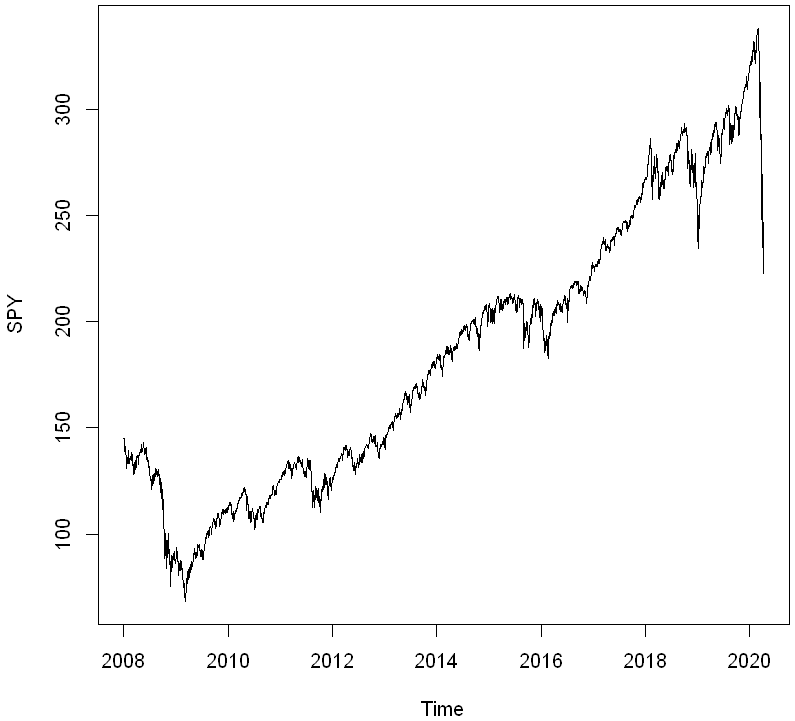
\includegraphics[width=0.95\textwidth]{output_3_0}
            \caption{08年后S\&P500的指数走势.\label{fig:1}}
        \end{figure}
    \end{minipage}
    \begin{minipage}{0.35\textwidth}
        \begin{figure}
            \centering
            \hspace{-25pt}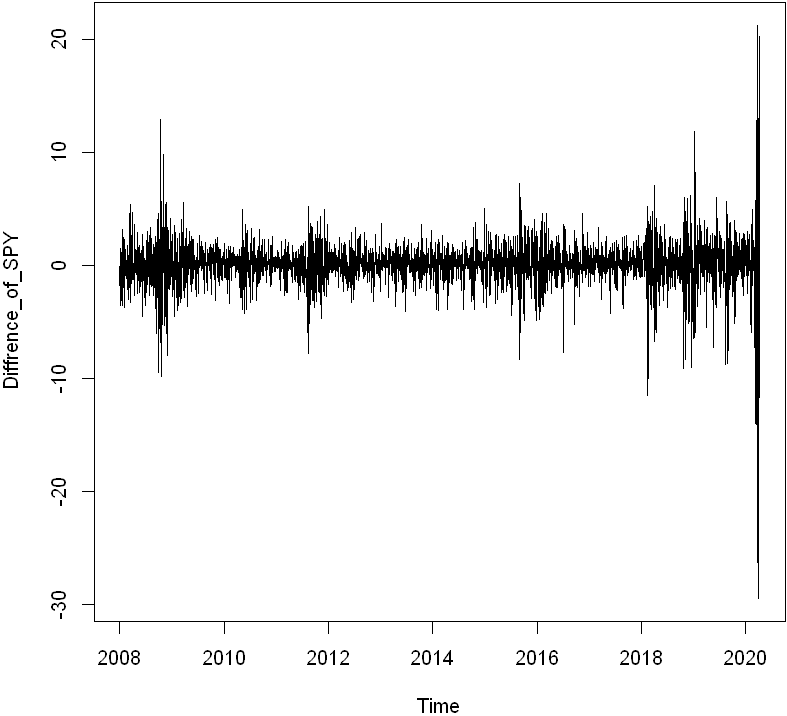
\includegraphics[width=0.95\textwidth]{output_4_0}
            \caption{S\&P500指数差分序列的图示.\label{fig:2}}
        \end{figure}
    \end{minipage}
\end{center}


从图 \ref{fig:1} 中, 可以明显的看出它有一定的趋势, 因而并非平稳序列. 故考虑它的一阶差分序列, 将其画出, 如图 \ref{fig:2}. 从中可以看出, 差分序列基本都是围绕着0上下波动的, 因此, 可以看作是弱平稳序列. 于是, 接下来对于一阶差分序列进行分析. 
\section{初步建模}
\qquad 首先对于差分序列实行$ADF$单位根检验, 结果如下
\begin{center}
    Dickey-Fuller = -14.196, Lag order = 14, p-value = 0.01. 
\end{center}
由此, 可以判断一阶差分序列是稳定的. 因此, 可以进行下一步分析. 
\subsection{定阶}
\qquad 之后需要确定ARIMA模型的阶数, 首先作出ACF和PACF图, 如图 \ref{fig:3} \ref{fig:4} 所示, 虚线表示的是两倍标准误差的上下界. 
\begin{center}
    \hspace{30pt}\begin{minipage}{0.35\textwidth}
        \begin{figure}
            \centering
            \hspace{-30pt}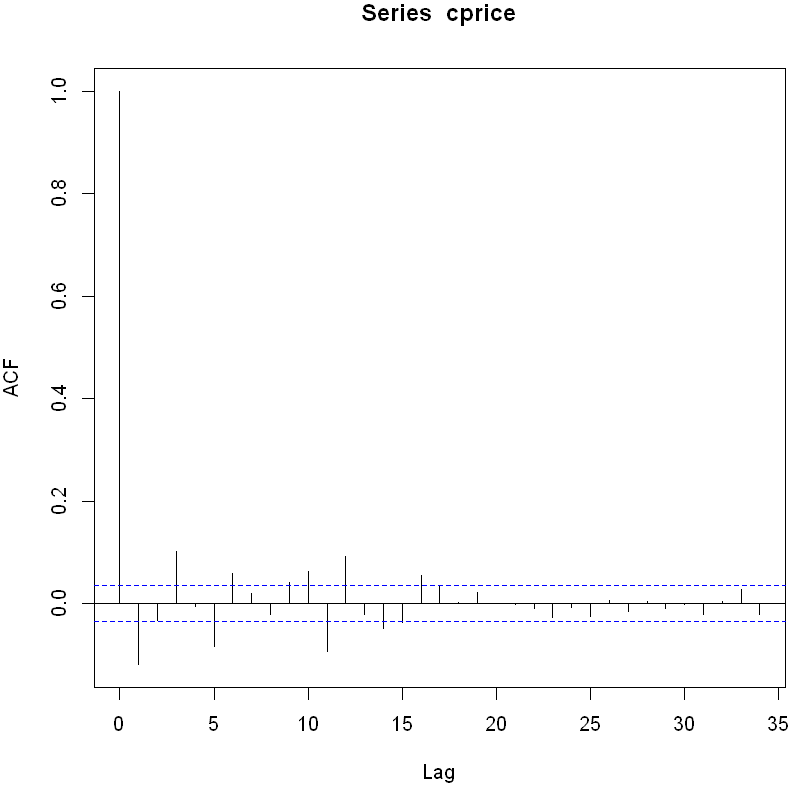
\includegraphics[width=.95\textwidth]{output_8_0}
            \caption{差分序列的$ACF$图.\label{fig:3}}
        \end{figure}
    \end{minipage}
    \begin{minipage}{0.35\textwidth}
        \begin{figure}
            \centering
            \hspace{-25pt}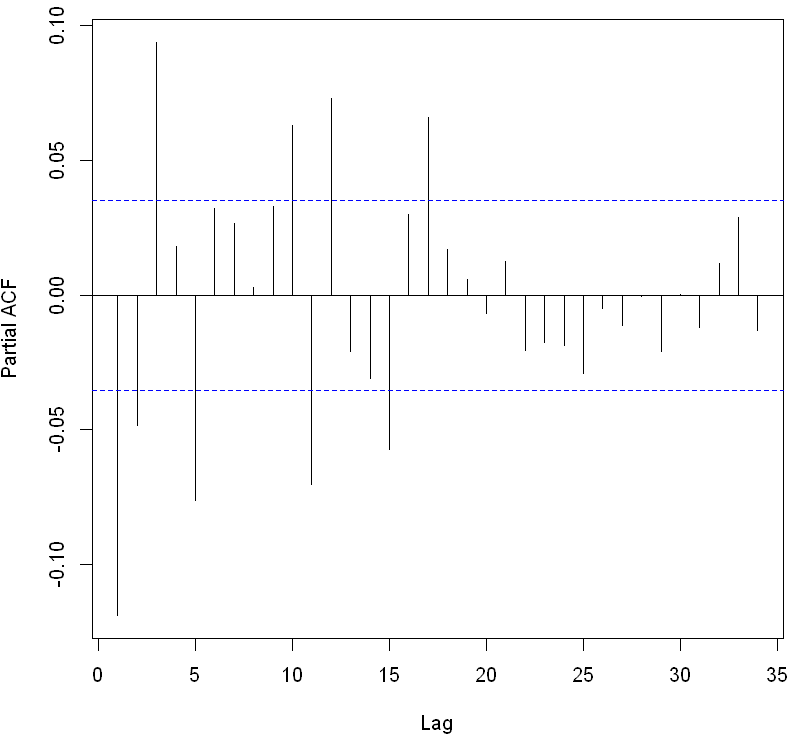
\includegraphics[width=.95\textwidth]{output_9_0}
            \caption{差分序列的$PACF$图.\label{fig:4}}
        \end{figure}
    \end{minipage}
\end{center}
\qquad 可以看出, 两个图像都存在拖尾现象, $p=4,q=4$是一组可能的解, 但无法确定确切的最优的 (p,q) 的值, $ACF$和$PACF$为识别纯$AR(p)$和$MA(q)$模型提供了有效的工具. 但对于混合$ARMA$模型来说, 它的理论$ACF$和$PACF$有着无限多的非零值, 这使得根据样本$ACF$和$PACF$来识别混合模型非常困难. 于是我们通过更适合大样本的$EACF$来进一步确定.
\begin{longtable}[c]{c|cccccccccccccc}
    \caption{EACF结果}
    \label{tab:my-table}\\
    \hline
    AR/MA & 0 & 1 & 2 & 3 & 4 & 5 & 6 & 7 & 8 & 9 & 10 & 11 & 12 & 13 \\ \hline
    \endfirsthead
    %
    \endhead
    %
    \hline
    \endfoot
    %
    \endlastfoot
    %
    0     & X & O & X & O & X & X & O & O & X & X & X  & X  & O  & X  \\
    1     & X & X & X & O & X & X & X & O & O & X & O  & X  & O  & O  \\
    2     & X & X & O & O & O & X & O & O & O & X & X  & X  & X  & O  \\
    3     & X & X & X & O & O & O & O & O & X & O & O  & X  & O  & O  \\
    4     & X & X & X & X & O & O & O & X & O & O & O  & X  & X  & O  \\
    5     & X & X & X & X & X & O & X & X & O & O & O  & X  & O  & X  \\
    6     & X & X & X & X & X & X & O & X & O & O & O  & X  & O  & O  \\
    7     & X & X & X & O & X & X & X & O & X & X & O  & X  & X  & O  \\ \hline
    \end{longtable}
由表\ref{tab:my-table} 可知, $p=2,q=3;p=2,q=6;p=3 q=4;p=3,q=5$时的ARMA模型可能比较合适. 

\qquad 使用赤池信息准则 (AIC) 对于模型的参数进行筛选, 此准则要求选择使下式最小化的模型\[
    AIC=-2\log(MLE) +2k.
\]
通过R自带的$auto.arima()$函数(此函数以$AIC$为准则)得到的推荐参数选择为$p=5,q=0$. 另外, 还可以使用Schwarz贝叶斯信息准则($BIC$)最来筛选参数, $BIC$定义如下的\[
    BIC= -2log(MLE)+klog(n).
\]
在此准则下各参数的$BIC$如图 \ref{fig:bic} 所示.
\begin{figure}
    \centering
    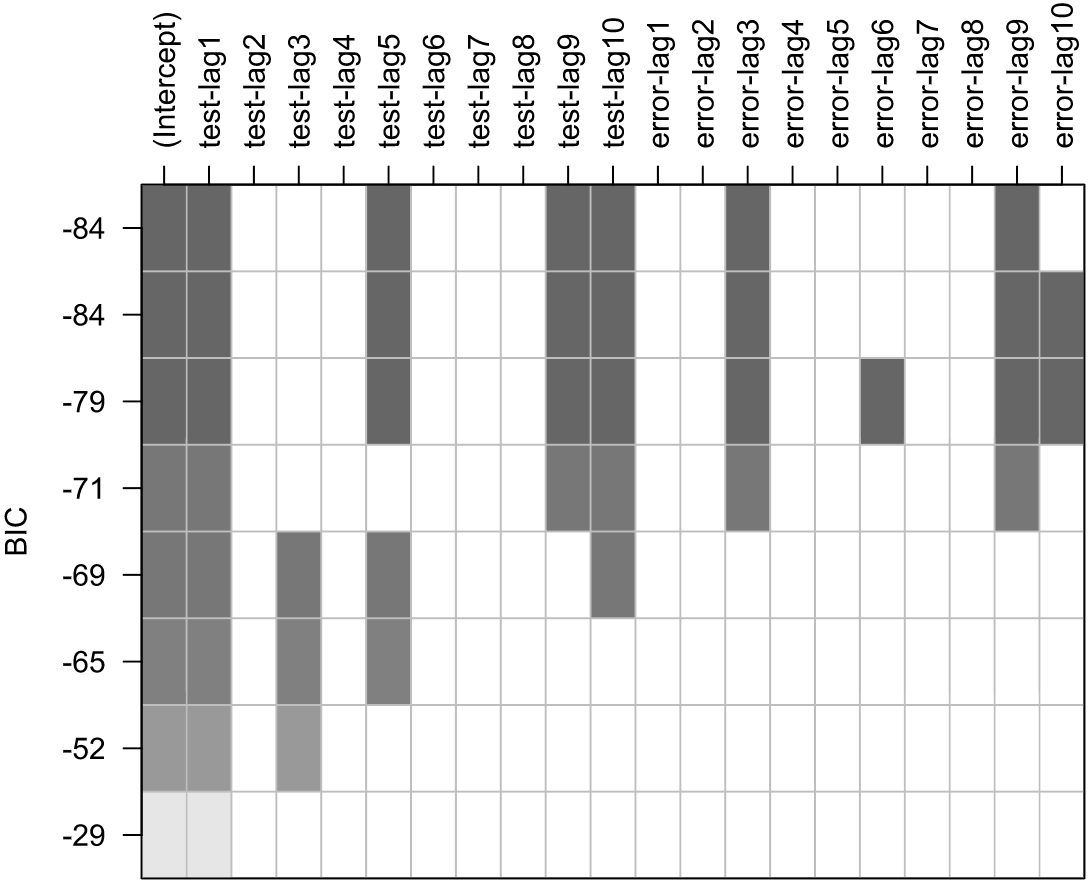
\includegraphics[width=.4\textwidth]{bic}
    \caption{最优子集结果. \label{fig:bic}}
\end{figure}

\qquad 从图中可以出, 应该使用$Y_{(t-1)},Y_{(t-5)},Y_{(t-9)},Y_{(t-10)}$来建模, 误差部分需要三阶和九阶滞后项. 但这样的话相关项会过多, 且结合ACF与PACF图, 发现在滞后项1、5、10上均比较大, 转而考虑是否存在季节性因素, 即将一周开盘的5天视为一个季节, 进行研究. 

\qquad 首先对价格隔五项进行差分, 画出$ACF, PACF$的图像, 如图 \ref{fig:acf1} \ref{fig:pacf1}.
\begin{center}
    \hspace{30pt}\begin{minipage}{0.45\textwidth}
        \begin{figure}
            \centering
            \hspace{-30pt}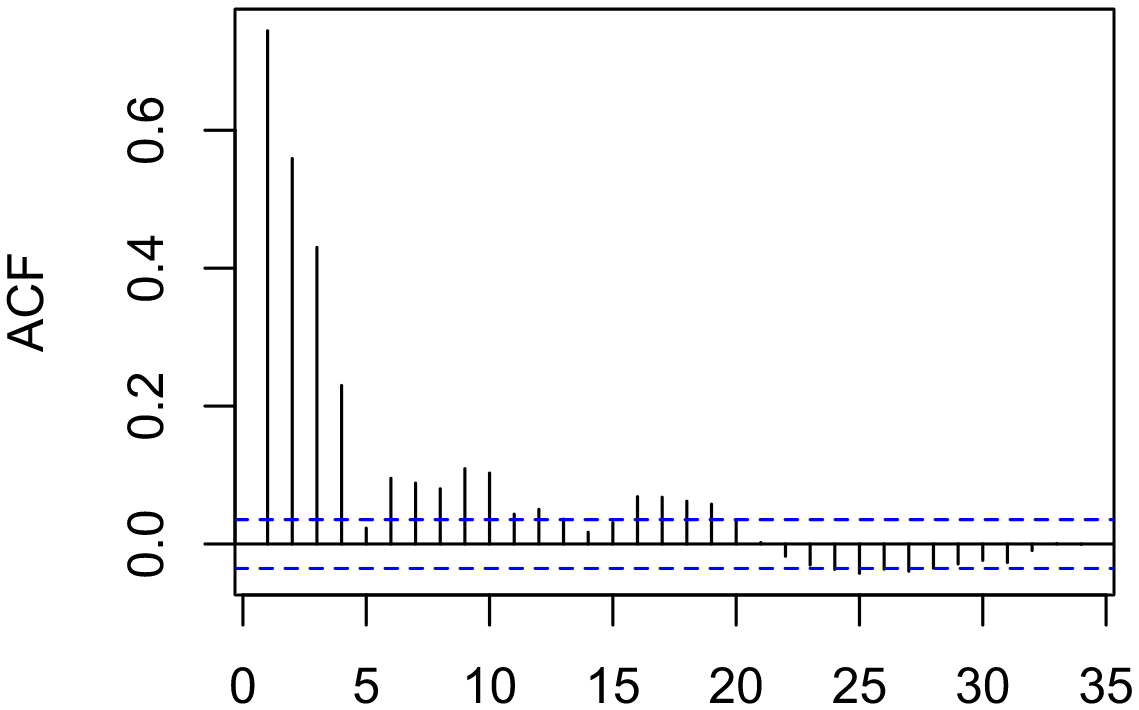
\includegraphics[width=.95\textwidth]{acf1}
            \caption{差分序列的$ACF$图.\label{fig:acf1}}
        \end{figure}
    \end{minipage}
    \begin{minipage}{0.45\textwidth}
        \begin{figure}
            \centering
            \hspace{-25pt}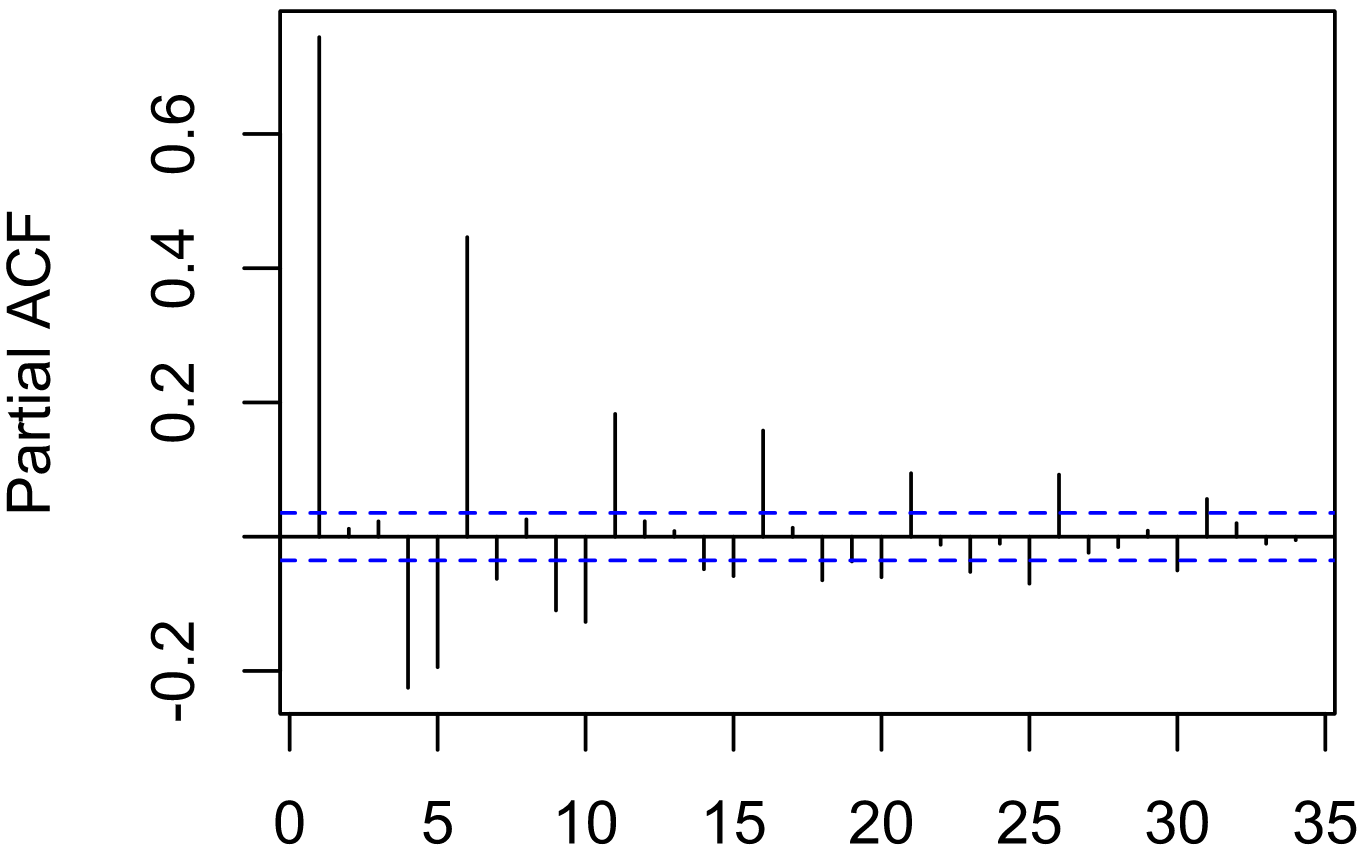
\includegraphics[width=.95\textwidth]{pacf1}
            \caption{差分序列的$PACF$图.\label{fig:pacf1}}
        \end{figure}
    \end{minipage}
\end{center}
\qquad 结合$ACF$和$PACF$图判断选择模型即可,为了排除偏差, 使用$P=1,P=2$都进行了实验,得到的AIC信息准则结果如表 \ref{tab:my-table2}. 
\begin{table}[htbp]
    \centering
    \caption{各种模型的AIC值}
    \label{tab:my-table2}
    \begin{tabular}{c|cccccccccccc}
    \hline
    p & 4 & 4 & 5 & 5 & 2 & 2 & 3 & 3 & 3 & 3 & 2 & 2 \\
    d & 1 & 1 & 1 & 1 & 1 & 1 & 1 & 1 & 1 & 1 & 1 & 1 \\
    q & 4 & 4 & 0 & 0 & 3 & 3 & 4 & 4 & 5 & 5 & 6 & 6 \\
    P & 1 & 2 & 1 & 2 & 1 & 2 & 1 & 2 & 1 & 2 & 1 & 2 \\
    D & 0 & 0 & 0 & 0 & 0 & 0 & 0 & 0 & 0 & 0 & 0 & 0 \\
    Q & 0 & 0 & 0 & 0 & 0 & 0 & 0 & 0 & 0 & 0 & 0 & 0 \\ \hline
    AIC值($13000+$) & 502 & 497 & 506 & 504 & 512 & 515 & 498 & 494 & 481 & 483 & 494 & 511 \\ \hline
    \end{tabular}
\end{table}

比较$AIC$后, 选择最小的$ARIMA(3,1,5)(1,0,0)[5]$进行建模. 
\subsection{模型建立}
\qquad 使用上文的$ARIMA(3,1,5)(1,0,0)[5]$进行建模, 得到的模型为
\[
    \textcolor{red}{\left(Y_t+0.1151 Y_{t-1}+ 0.0337Y_{t-2}-0.0943 Y_{t-3}\right)\left(Y_t+0.0708Y_{t-1}-0.0625Y_{t-2}\right)=\varepsilon_t,\ \varepsilon_t\sim N(0,1).}
\]
并且画出模型的单位根的分布, 如图 \ref{fig:m1r}.
\begin{figure}[htbp]
    \centering
    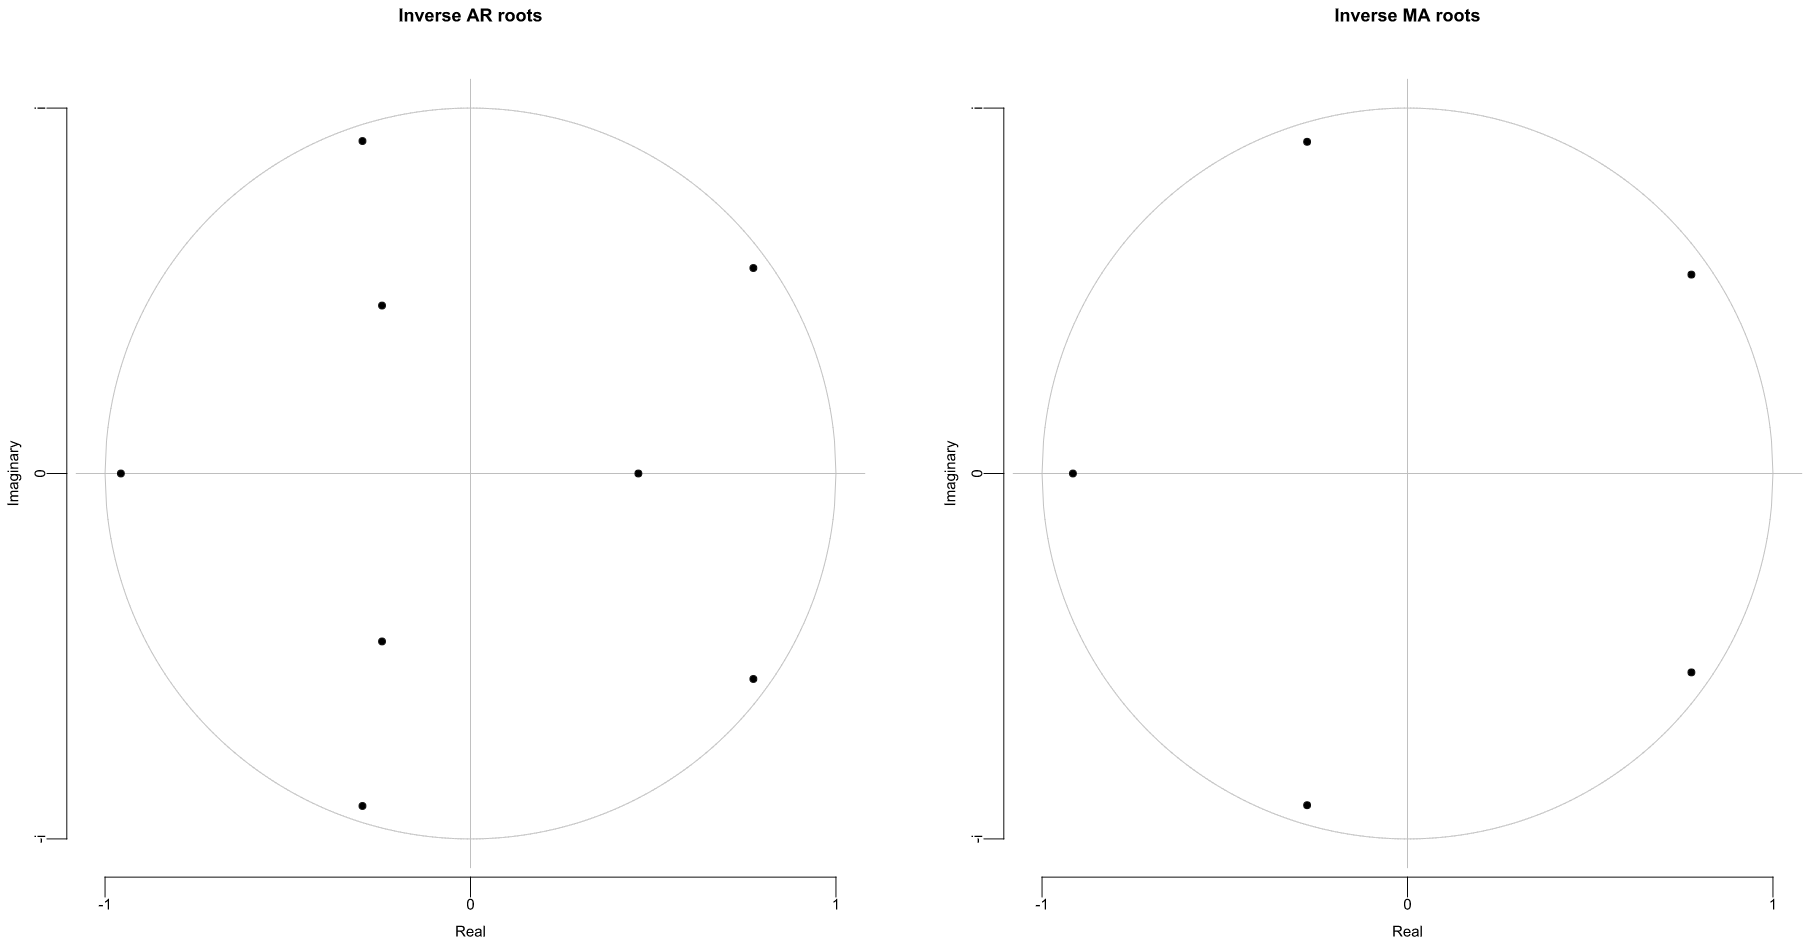
\includegraphics[width=.85\textwidth]{m1}
    \caption{模型的单位根分布. \label{fig:m1r}}
\end{figure}

同时, 画出残差的分布, 如图 \ref{fig:m1res1}.

\begin{center}
    \hspace{-10pt}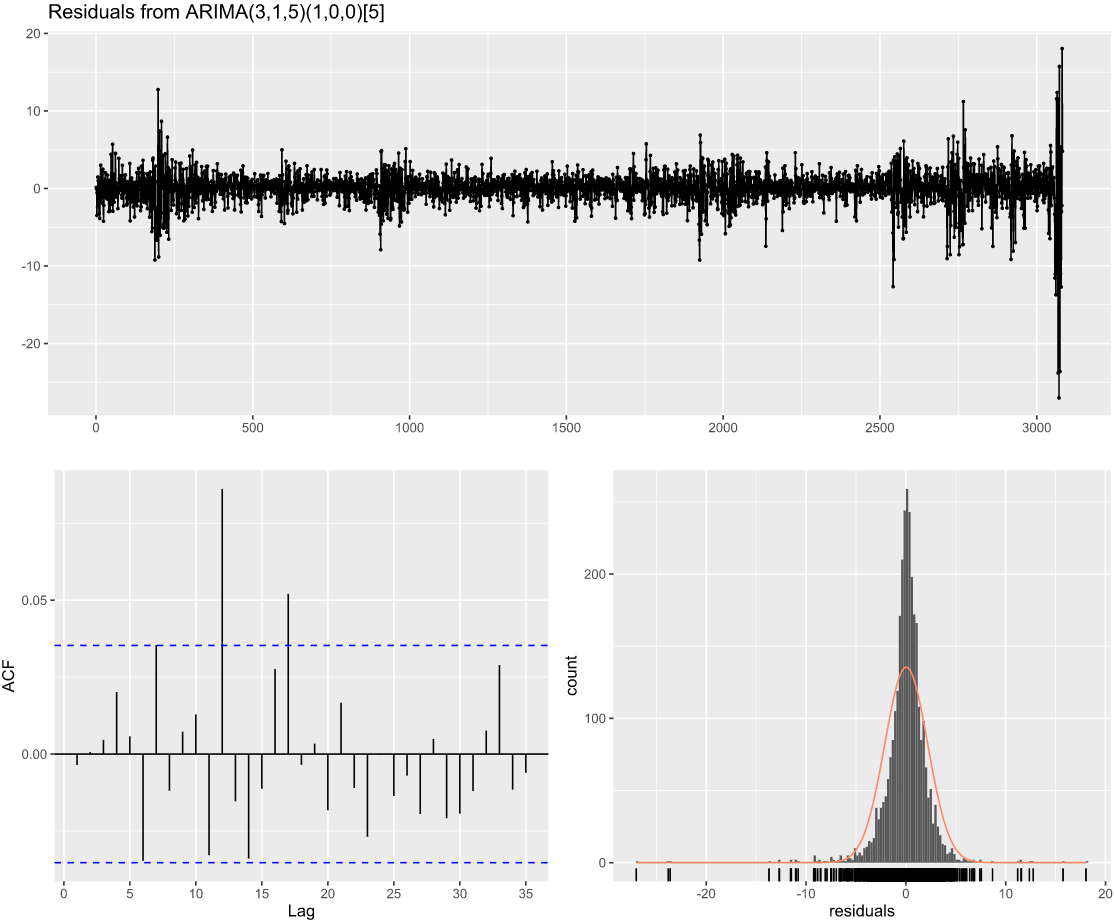
\includegraphics[width=.8\textwidth]{m1res1}
\end{center}
\begin{figure}[htbp]
    \centering
    \caption{残差的分布. \label{fig:m1res1}}
\end{figure}

\qquad 可以看到, 单位根都在单位圆内, 同时, 对与残差进行Ljung-Box检验, 结果如下
\begin{center}
    Q* = 36.489, df = 3, p-value = 5.902e-08.
\end{center}
$p$值接近0, 因此, 残差的正态性相当好, 但通过残差的$ACF$图可以看出模型仍不是十分理想. 接下来使用此模型对于未来的走势进行预测, 预测结果如图 \ref{fig:7}.
\begin{figure}
    \centering
    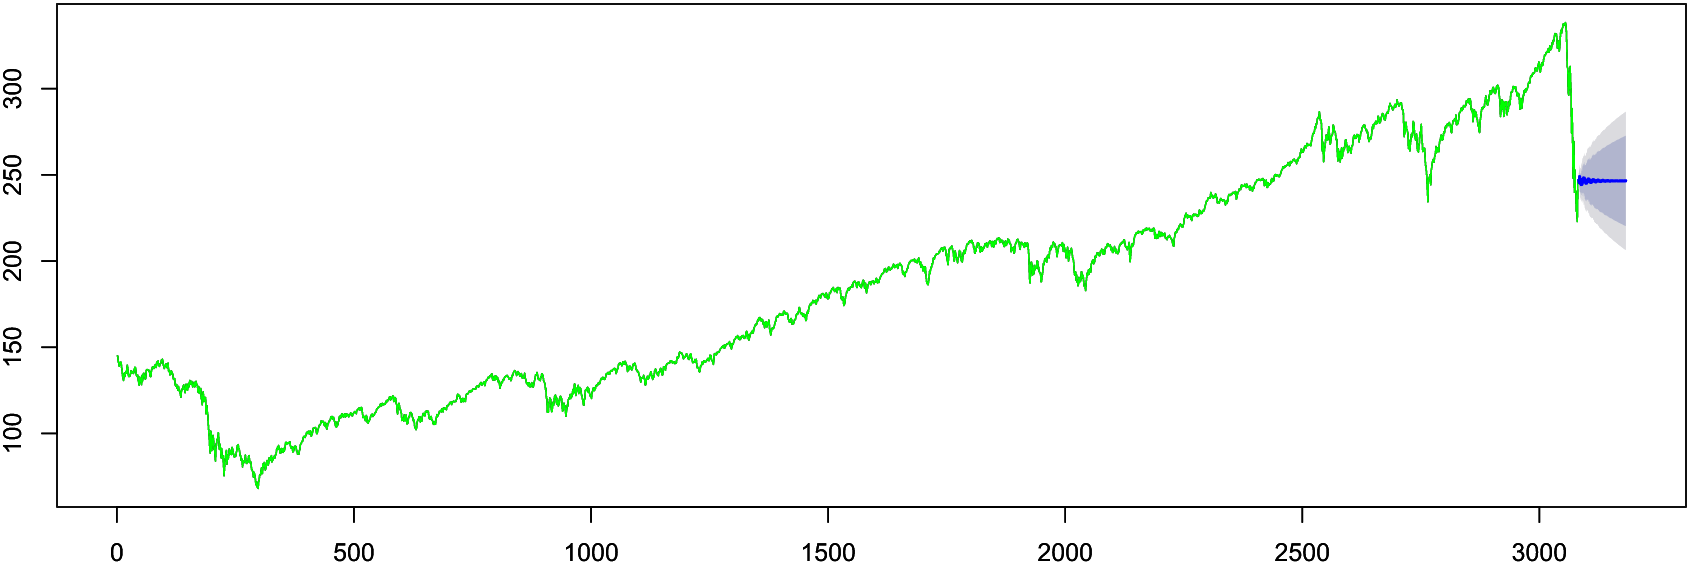
\includegraphics[width=.82\textwidth]{f}
    \caption{模型预测结果. \label{fig:7}}
\end{figure}







\section{剔除季节因素}
\subsection{拟合纯季节模型}
\qquad 价格可能会受到季节性的影响, 并且数据为股票市场, 因此可以合理地假设这个周期现象为周模式, 因为一周有五个工作日, 故先对于价格差分序列拟合一个纯季节模型. 其中, 先计算了$P=1,2,3$时的$AIC$, 如表 \ref{tab:my-table3}. 
\begin{table}[htbp]
    \centering
    \caption{纯季节模型的$AIC$.}
    \label{tab:my-table3}
    \begin{tabular}{c|ccc}
    \hline
    P   & 1        & 2        & 3        \\ \hline
    AIC & 13588.65 & 13580.55 & 13579.58 \\ \hline
    \end{tabular}
\end{table}

由此, 选择$P=3$, 得到的模型$b_t$如下
\[
    b_t=(1+0.0790L^5-0.0651L^{10}+0.0373L^{15})Y_t.  
\]
同样, 画出它的单位根的分布与残差的图像, 如图 \ref{fig:8} \ref{fig:9}.
\begin{center}
    \hspace{30pt}\begin{minipage}{0.45\textwidth}
        \begin{figure}
            \centering
            \hspace{-30pt}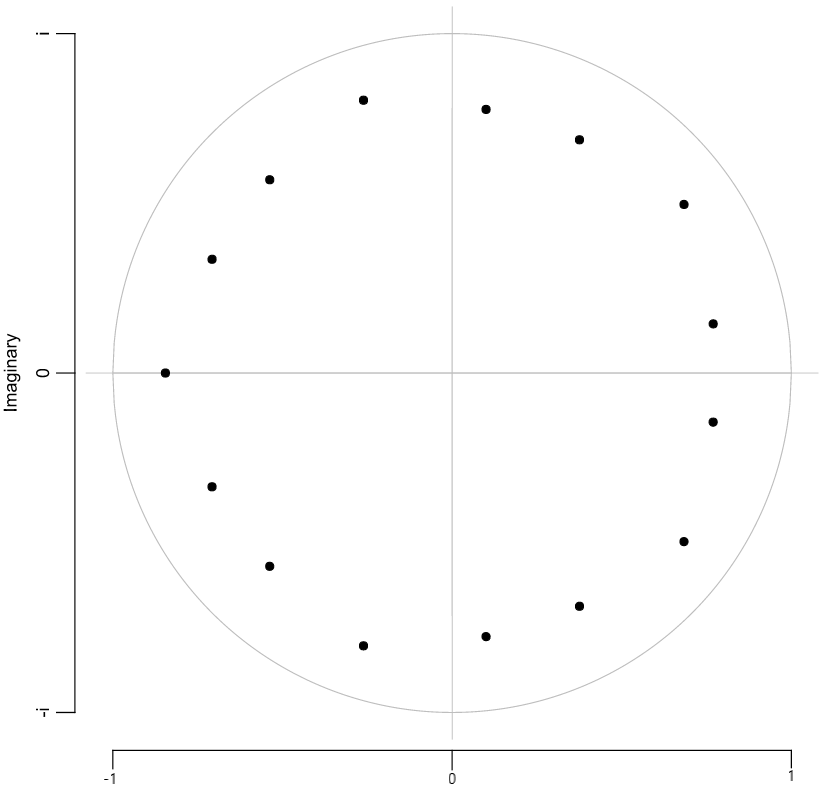
\includegraphics[width=.9\textwidth]{m2}
            \caption{单位根的分布.\label{fig:8}}
        \end{figure}
    \end{minipage}
    \begin{minipage}{0.45\textwidth}
        \begin{figure}
            \centering
            \hspace{-25pt}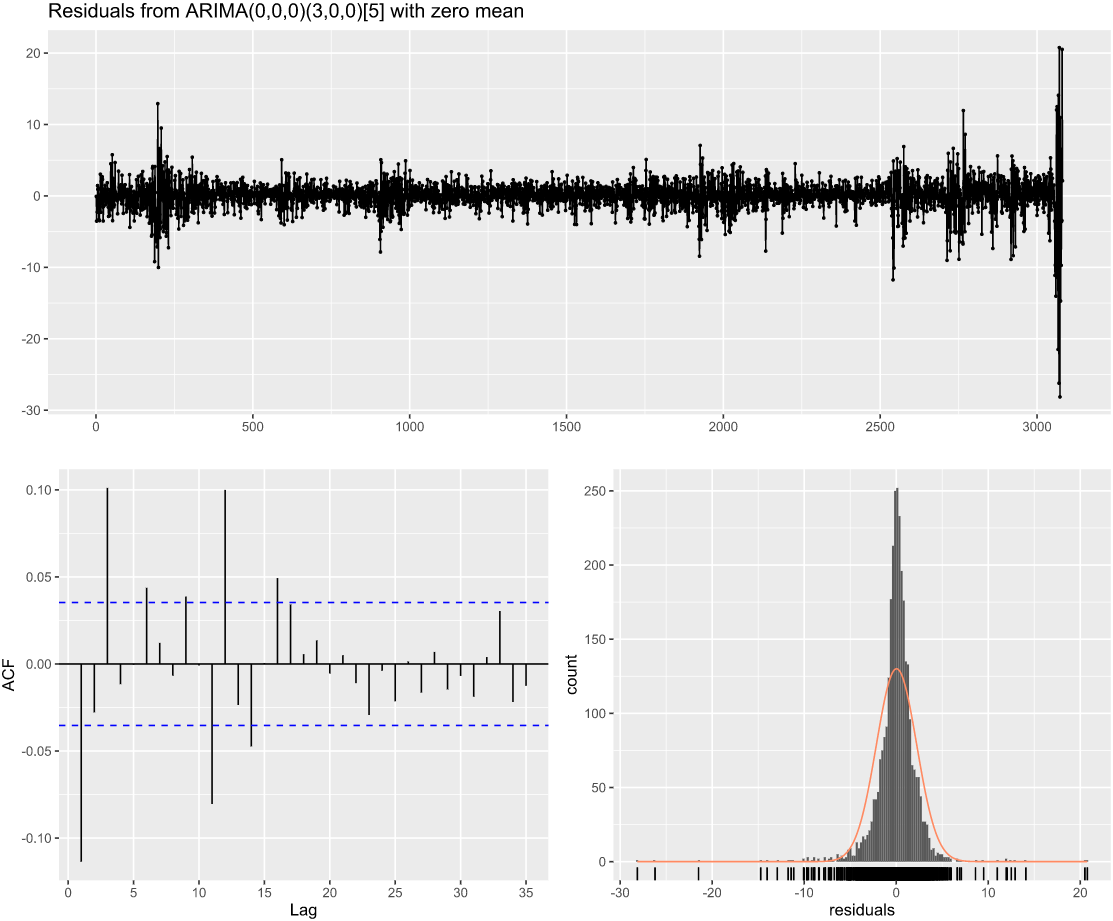
\includegraphics[width=.9\textwidth]{m21}
            \caption{模型残差的分布.\label{fig:9}}
        \end{figure}
    \end{minipage}
\end{center}
    
\qquad 可以看到单位根均在单位圆之内, 因此是平稳的. 但从$ACF$序列中也可以看出纯季节性的模型并不理想. 
\subsection{剔除季节性影响}








\qquad 之后, 对于$Y_t$, 结合春季节性模型进行调整
\[
    Y_t^*=Y_t+0.0790Y_{t-5}-0.0651Y_{t-10}+0.0373L_{t-15}, t=16,17,\cdots,3071.
\]

首先对调整后的序列做分析, 画出其自相关与偏自相关图像如图 \ref{fig:11} \ref{fig:12}. 

\begin{center}
    \hspace{30pt}\begin{minipage}{0.45\textwidth}
        \begin{figure}
            \centering
            \hspace{-25pt}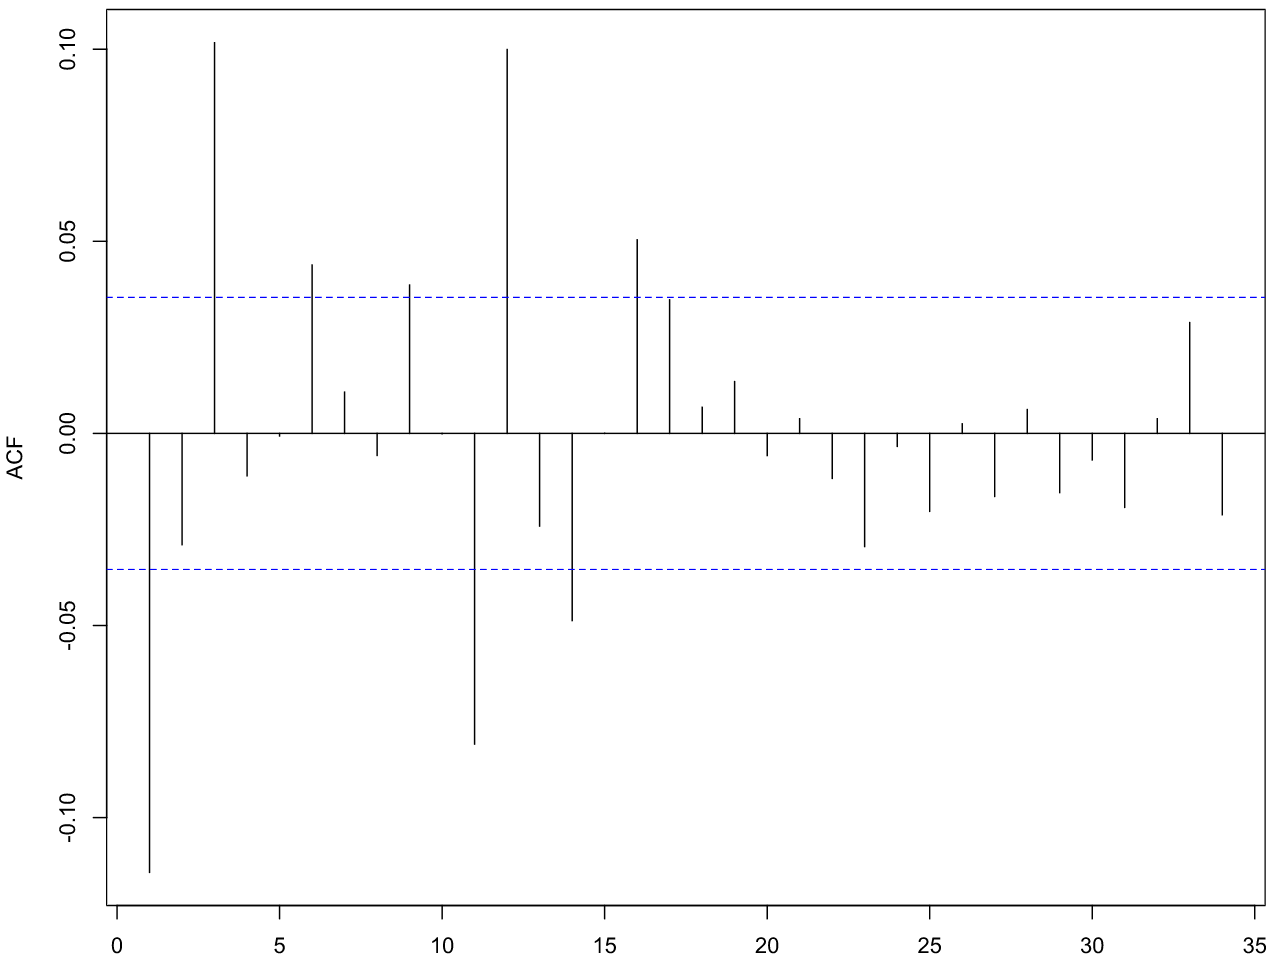
\includegraphics[width=.9\textwidth]{acf2}
            \caption{调整后的差分序列$ACF$图.\label{fig:11}}
        \end{figure}
    \end{minipage}
    \begin{minipage}{0.45\textwidth}
        \begin{figure}
            \centering
            \hspace{-25pt}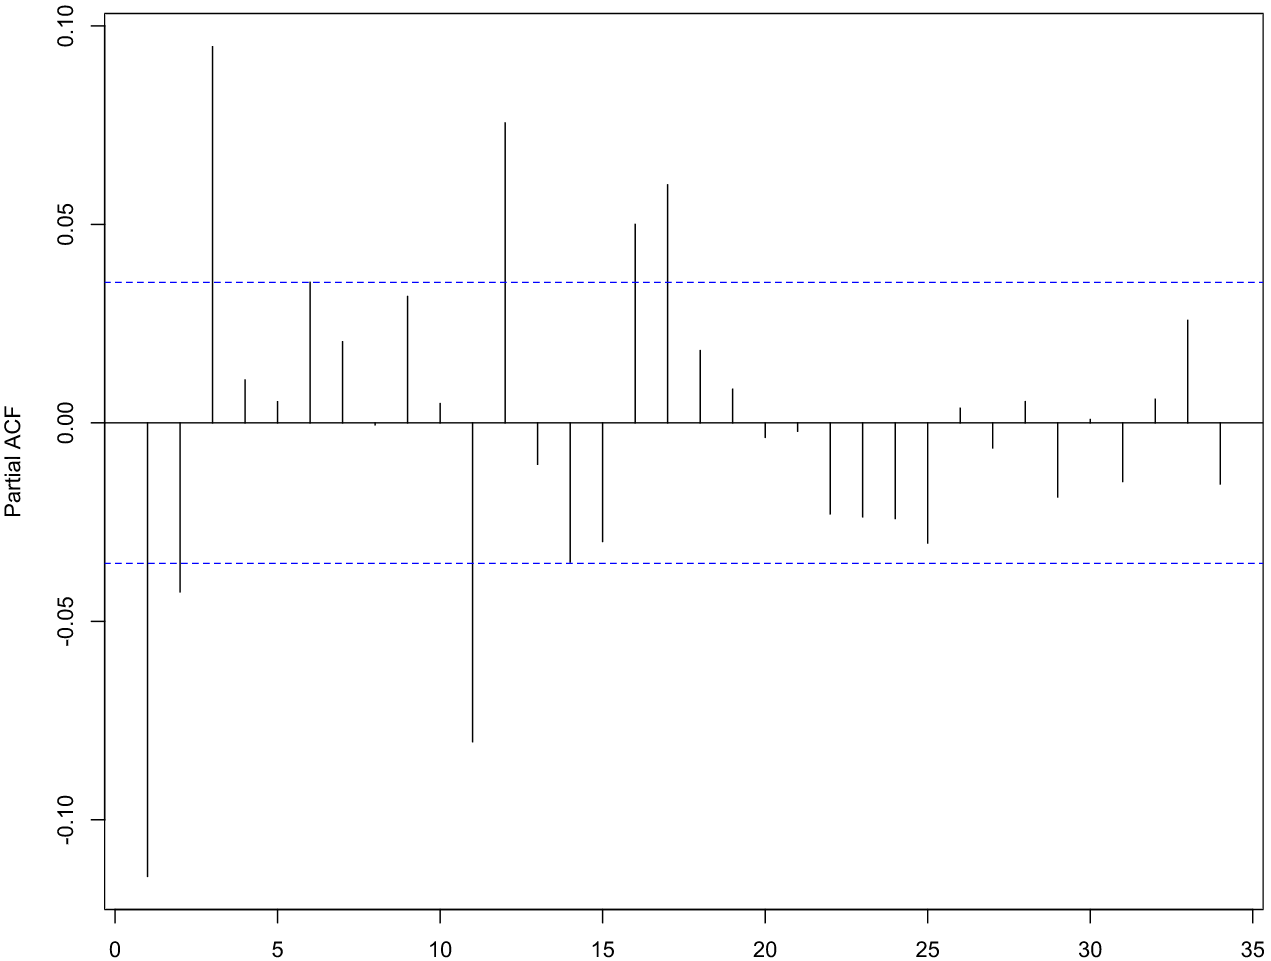
\includegraphics[width=.9\textwidth]{pacf2}
            \caption{调整后的差分序列$PACF$图.\label{fig:12}}
        \end{figure}
    \end{minipage}
\end{center}

\qquad 可以看出, 相比于原来的$ACF$与$PACF$图像, 调整后的价格在5,10阶上已有大大的下降, 因此, 可以说我们较为成功地剔除了季节性的影响. 
\section{结合GARCH模型}
\qquad GARCH模型允许波动率随着时间进行变化, 并且允许波动率的聚集. 即在随机项$\epsilon_t$前的系数并非像ARMA一样为一个常数, 而是一个与时间相关的函数$\sigma_t$. 因此, 我们需要对这个函数进行建模. GARCH对这个系数的建模是十分类似于ARMA模型对于价格的建模的. 如果对数收益表示为$r_t=\mu_t+a_t=\mu_t+\sigma_t\epsilon_t$, 那么GARCH(1,1)则为
\begin{equation*}
\sigma_t^2=\alpha_0+\alpha_1\alpha_{t-1}^2+\beta_1\sigma^2_{t-1}
\end{equation*}

\qquad 因为这样的波动率从确定的值变成了一个函数, 就可以用来模拟市场大起大落扎堆的现象, 能够对市场的变化响应得比ARMA模型更灵敏.

\qquad 我们猜想数据会受到多方面的外部因素的扰动, 所以对较长时间的数据分析十分的困难. 从数据分析中, 可以看出我们的差分序列波动的最大程度既是价格上涨与下跌最明显的时候. ARMA模型无法处理这样的波动现象. 于是结合了GARCH模型来解释数据, 提高模型的预测能力. 

\subsection{使用GARCH初次建模}
\qquad 首先使用ARMA(3,0)+GARCH(1,1)对于调整后的价格序列进行建模. 拟合的模型为
\textcolor{red}{
\begin{equation*}\begin{aligned}
    Y_{t}^{*} &=-0.0428 Y_{t-1}^{*}-0.0062 Y_{t-2}^{*}-0.0104 Y_{t-3}^{*}+a_{t}, \quad a_{t}=\sigma_{t} \varepsilon_{t}, \quad \varepsilon_{t} \sim N(0,1) \\
    \sigma_{t}^{2} &=0.1035+ 0.1449 a_{t-1}^{2}+0.8288 \sigma_{t-1}^{2}
\end{aligned}\end{equation*}}
同时还发现$ARMA$的第一个系数比较显著. 

\qquad 为了进一步的改进模型, 使用残差的相关图像对模型进行了可视化. 结果如图 \ref{fig:13} \ref{fig:14}.
\begin{center}
    \hspace{30pt}\begin{minipage}{0.45\textwidth}
        \begin{figure}
            \centering
            \hspace{-25pt}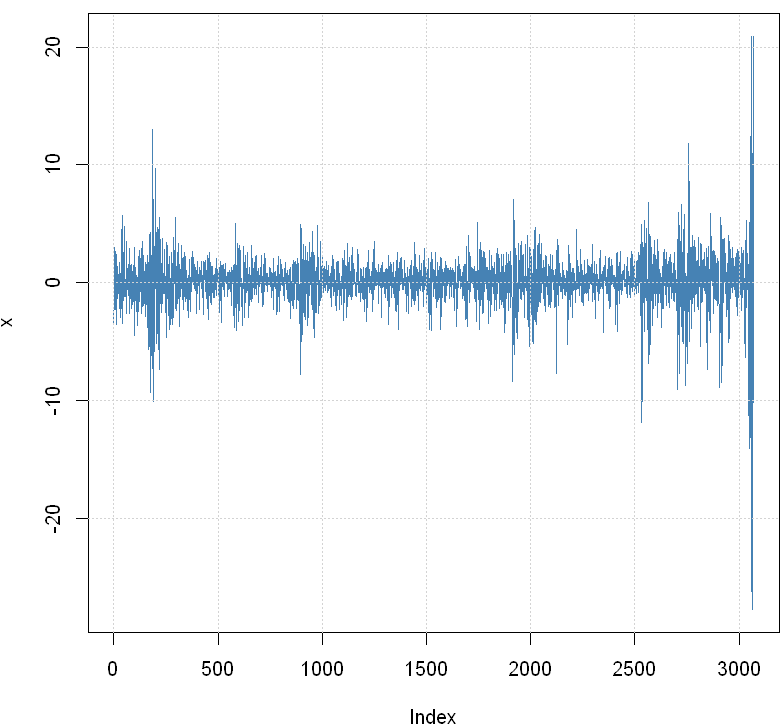
\includegraphics[width=.9\textwidth]{output_36_0}
            \caption{模型所拟合的时间序列.\label{fig:13}}
        \end{figure}
    \end{minipage}
    \begin{minipage}{0.45\textwidth}
        \begin{figure}
            \centering
            \hspace{-25pt}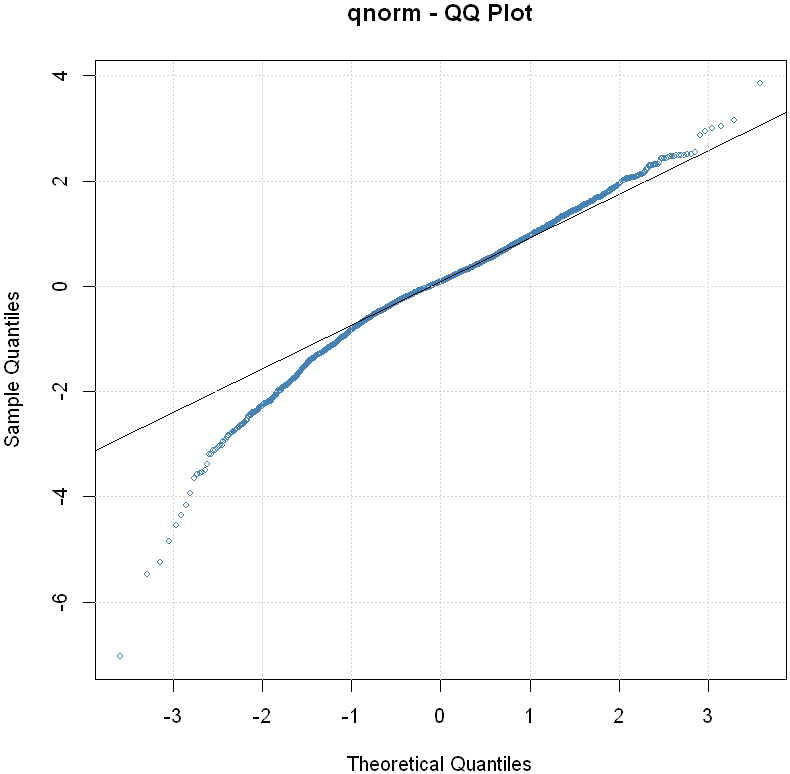
\includegraphics[width=.9\textwidth]{output_37_0}
            \caption{残差值与正态分布的QQ图.\label{fig:14}}
        \end{figure}
    \end{minipage}
\end{center}
    
\qquad 可以明显地看到, 标准化残差的正态性并不是十分的好, 因此模型还需进一步的调整.

\subsection{新息分布更换}
\qquad 改进的模型与上一个模型基本相同, 但是考虑了不同的新息分布. 采用了t分布作为新的新息分布. 模型如下
\textcolor{red}{
\begin{equation*}\begin{aligned}
    Y_{t}^{*} &=-0.0395 Y_{t-1}^{*}-0.0047 Y_{t-2}^{*}-0.0035 Y_{t-3}^{*}+a_{t}, \quad a_{t}=\sigma_{t} \varepsilon_{t}, \quad \varepsilon_{t} \sim N(0,1) \\
    \sigma_{t}^{2} &=0.0739+ 0.1349 a_{t-1}^{2}+0.8516 \sigma_{t-1}^{2}
\end{aligned}\end{equation*}}

\qquad 从结果可以看到, 依旧只有$ARMA$的第一个系数比较显著, 同时, 对新息的假设也通过了$L-B$检验. 同样的, 我们对于残差的分布进行可视化. 如图 \ref{fig:15} \ref{fig:16}.

\begin{center}
    \hspace{30pt}\begin{minipage}{0.45\textwidth}
        \begin{figure}
            \centering
            \hspace{-25pt}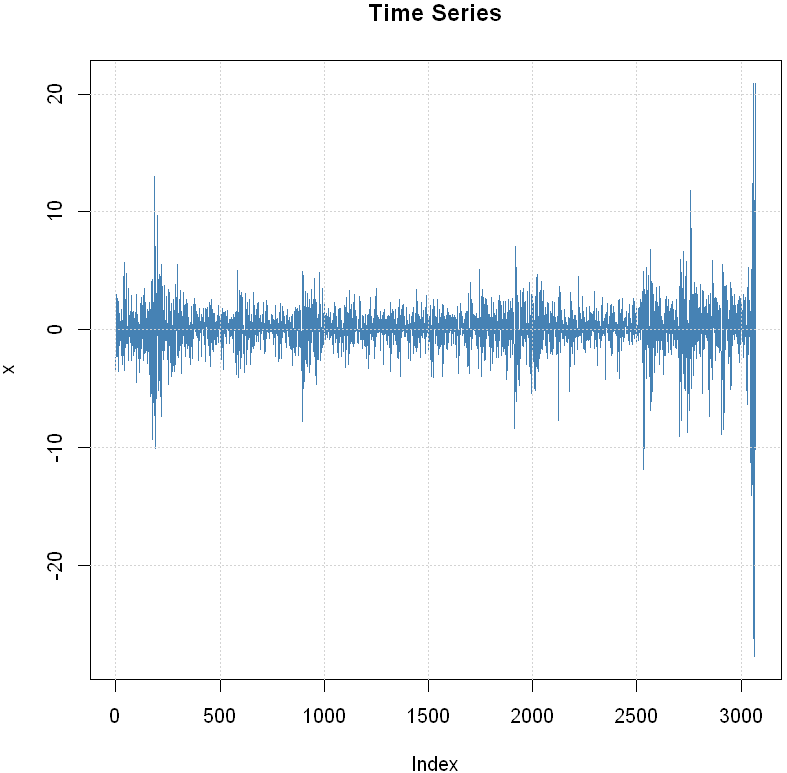
\includegraphics[width=.9\textwidth]{output_44_0}
            \caption{模型所拟合的时间序列.\label{fig:15}}
        \end{figure}
    \end{minipage}
    \begin{minipage}{0.45\textwidth}
        \begin{figure}
            \centering
            \hspace{-25pt}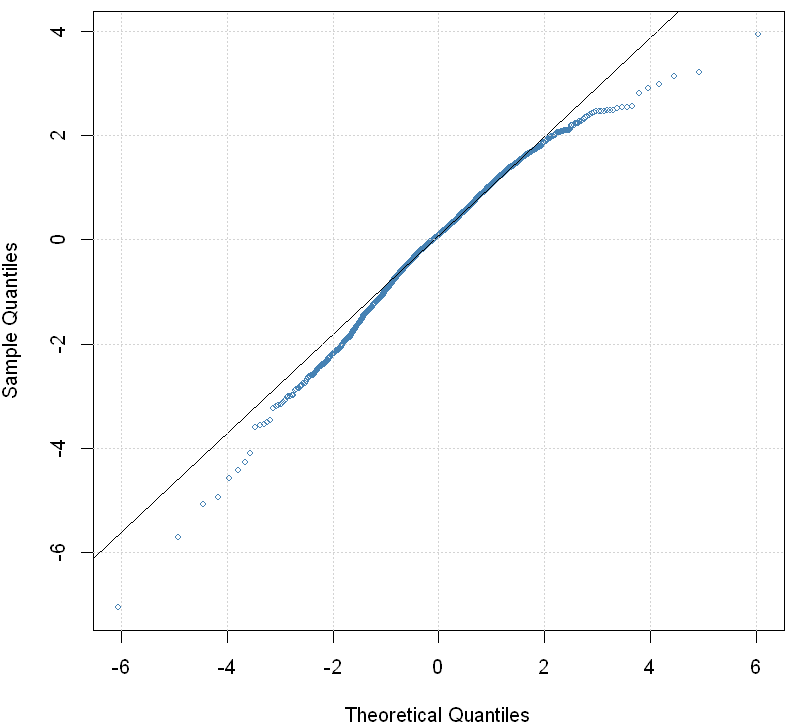
\includegraphics[width=.9\textwidth]{output_45_0}
            \caption{残差值与正态分布的QQ图.\label{fig:16}}
        \end{figure}
    \end{minipage}
\end{center}

\qquad 从图中可以发现, 此时模型的效果反而变差了. 标准化残差的分布依旧左偏, 并且左偏得更加严重. 因此, 需要更新对于新息分布的假设. 自然而然的就考虑了能够处理这样情况的偏t分布.

\subsection{缩减$ARMA$的系数个数}
\qquad 由于前两次的模型除了$MA$的第五个系数并不显著性. 因此, 考虑将模型更换到$ARMA(3,4)+GARCH(1,1)$. 并且采用偏t分布作为新息分布. 拟合的模型如下
\textcolor{red}{
\begin{equation*}\begin{aligned}
    Y_{t}^{*} &=-0.0631 Y_{t-1}^{*}+a_{t}, \quad a_{t}=\sigma_{t} \varepsilon_{t}, \quad \varepsilon_{t} \sim N(0,1) \\
    \sigma_{t}^{2} &=0.0729+ 0.1329 a_{t-1}^{2}+ 0.8554 \sigma_{t-1}^{2}
\end{aligned}\end{equation*}}

\qquad 在这个模型中, $ARMA$的七个系数的显著性全部十分的高. 残差的分布可视化如图 \ref{fig:17} \ref{fig:18}.
\begin{center}
    \hspace{30pt}\begin{minipage}{0.45\textwidth}
        \begin{figure}
            \centering
            \hspace{-25pt}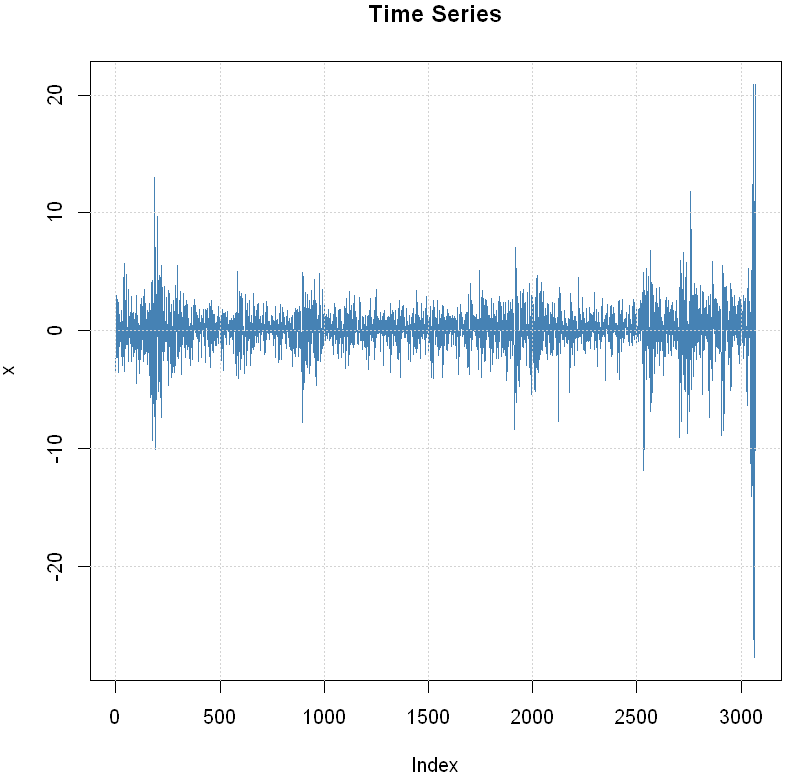
\includegraphics[width=.9\textwidth]{output_52_0}
            \caption{模型所拟合的时间序列.\label{fig:17}}
        \end{figure}
    \end{minipage}
    \begin{minipage}{0.45\textwidth}
        \begin{figure}
            \centering
            \hspace{-25pt}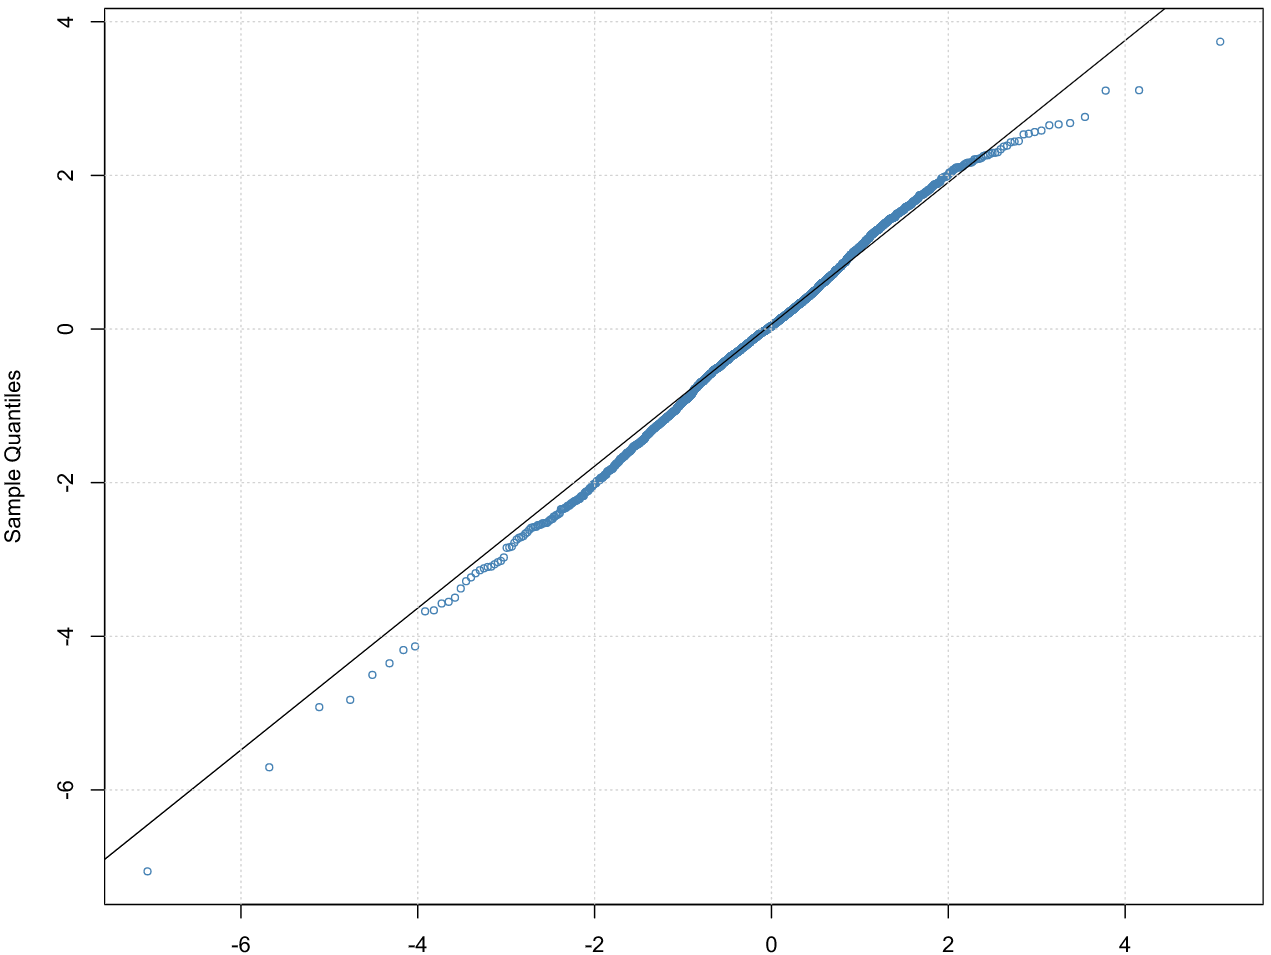
\includegraphics[width=.9\textwidth]{output_53_0}
            \caption{残差值与正态分布的QQ图.\label{fig:18}}
        \end{figure}
    \end{minipage}
\end{center}

\qquad 可以看到, 绝大部分点在该图中都表现出了一条直线的特征. 故可以认为偏t分布的假设对于新息而言是十分合理的, 虽然还是有轻微的左偏性.

\qquad 接下来, 对超前两步的数值进行预测, 结果如下

\begin{center}
    \begin{tabular}{ccccc}
 meanForecast & meanError & standardDeviation & lowerInterval & upperInterval\\
\hline
-2.932209 & 12.40724 & 12.40724  & -29.91137 & 19.32762\\                       
1.069844 & 12.36999 & 12.34532 & -25.82832 & 23.26285\\
\end{tabular}
\end{center}

\qquad 可以看到, 模型预测的$95\%$置信区间基本上处于调整后差分序列两个极值附近. 因为采用的是偏t分布, 所以区间并未呈现对称性. 反而是差分为正的置信区间更短, 意味着估计的确定性更高, 也就意味着我们对于未来的市场应该保持一个比较积极乐观的态度. 
\section{指数模型}
\qquad 指数模型是用来预测时序未来值时最常用的一种模型. 经过观察可以发现$2008\sim2019$年的S\&P$500$指数整体呈上升趋势, 因此可以使用指数模型对其进行拟合. 

\qquad 不同指数模型在建模过程中选用的因子不同. 如单指数模型(simple exponential model)拟合的只是常数水平项和时间点$i$处随机项的时间序列, 即认为时间序列不存在趋势项和季节效应; 双指数模型(double exponential model)也叫Holt指数平滑, 拟合的是有水平项和趋势项的时序; 三指数模型(triple exponential model)拟合的是有水平项、趋势项以及季节效应的时序. 

\qquad R中的ets()函数有自动选取对原始数据拟合优度最高的模型的功能, 因此, 我们使用拟合优度最高的方式, 获得如图 \ref{fig:20} 所示的结果.
\begin{figure}
    \centering
    \hspace{-30pt}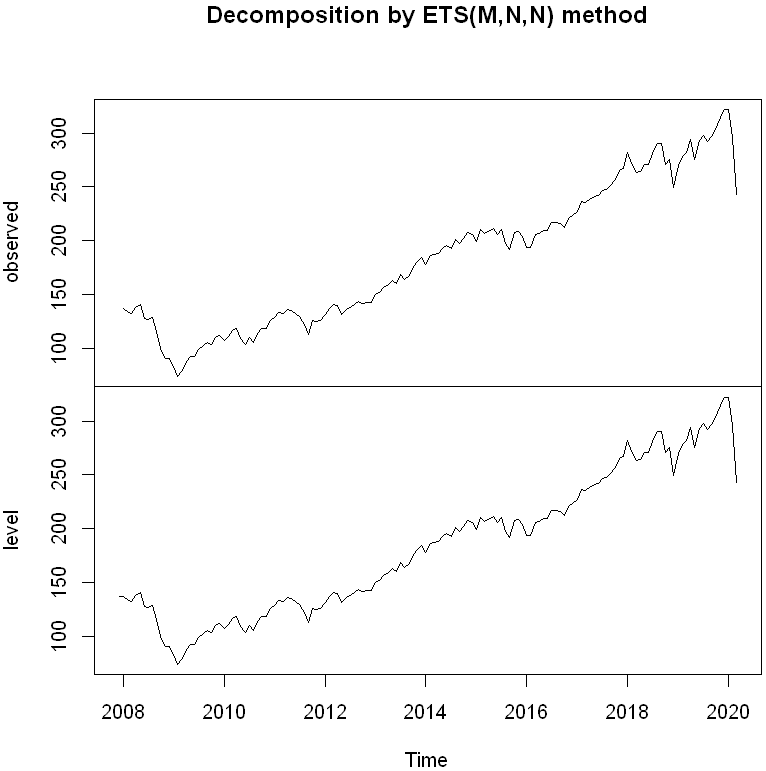
\includegraphics[width=.8\textwidth]{output_60_0}
    \caption{指数模型的结果.\label{fig:20}}
\end{figure}
\qquad 由于ets()的预测frequency的最大选择为24, 所以原数据直接采用了每月的S\&P500指数. 可以看到, 最终结果为$ETS(M,N,N), \alpha=0.99$, 即代表了单指数相乘模型. 而$\alpha$参数控制权重下降的速度, $\alpha$越接近1, 近期观测值的权重越大; 反之, 越接近于0, 则历史观测值的权重越大. 也就是
\[Y_t=level+irregular_r.\]

\qquad 单指数平滑根据现有的时序值的加权平均对未来做短期预测, 图 \ref{fig:21} 给出了其折线图和以下八个季度的预测. 
\begin{figure}
    \centering
    \hspace{-30pt}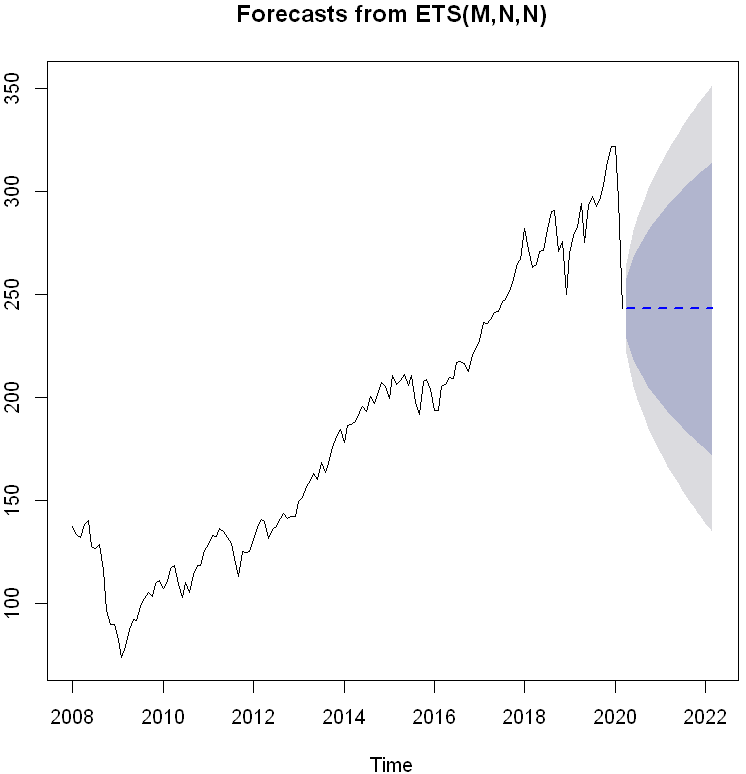
\includegraphics[width=.8\textwidth]{output_62_0}
    \caption{\footnotesize 可乘的单指数光滑预测, 其中预测值由虚线表示, $80\%$和$95\%$置信区间分别由淡灰色和深灰色表示.\label{fig:21}}
\end{figure}

\vspace{-10pt}\qquad 同时, 模型的各个度量标准如下

\ 

\begin{center}
\begin{tabular}{r|ccccccc}
  & ME & RMSE & MAE & MPE & MAPE & MASE & ACF1\\
\hline
	Training set & 0.7217255 & 8.607849 & 5.926743 & 0.2795169 & 3.445388 & 0.2628449 & 0.0787231\\
\end{tabular}
\normalsize
\end{center}

\ 

\qquad 一般来说由于平均误差和平均百分比会正向负向相抵消, 所以用处不大, RMSE给出了平均误差平方和平方根, 由于单指数模型相对简单易行, 即这样的误差水平还算令人满意. 
\section{结语}
\qquad 本文中我们采用了ARIMA、ARMA+GARCH、指数相乘三个模型对S\&P500进行研究, 在ARIMA与ARMA+GARCH中我们都试图通过去除季节性因素使预测更为准确, 并且对残差进行了正态性分析. 而对于新息的预测都是偏向积极, 即目前市场应该会慢慢回温. 在实验过程中, 我们也运用了一些自己并不是很熟悉的知识, 可能会存在使用理解有差或者使用不当的情况, 但这也是我们学习与探索的过程. 










































\newpage
\nocite{*}
\bibliographystyle{unsrt}
\bibliography{wpref}
\addcontentsline{toc}{section}{7\ \ \,参考文献}
\appendix
\section{完整代码}
\tiny
\begin{tcolorbox}[breakable, size=fbox, boxrule=1pt, pad at break*=1mm,colback=cellbackground, colframe=cellborder]
\prompt{In}{incolor}{1}{\boxspacing}
\begin{Verbatim}[commandchars=\\\{\}]
\PY{c+c1}{\PYZsh{} 加载所要用到的包}
\PY{n+nf}{library}\PY{p}{(}\PY{n}{fGarch}\PY{p}{)}
\PY{n+nf}{library}\PY{p}{(}\PY{n}{tseries}\PY{p}{)}
\PY{n+nf}{library}\PY{p}{(}\PY{n}{TSA}\PY{p}{)}
\PY{n+nf}{library}\PY{p}{(}\PY{n}{forecast}\PY{p}{)}
\PY{n+nf}{library}\PY{p}{(}\PY{n}{scales}\PY{p}{)}
\PY{n+nf}{library}\PY{p}{(}\PY{n}{plyr}\PY{p}{)}
\PY{n+nf}{library}\PY{p}{(}\PY{n}{TTR}\PY{p}{)}
\end{Verbatim}
\end{tcolorbox}
    \begin{tcolorbox}[breakable, size=fbox, boxrule=1pt, pad at break*=1mm,colback=cellbackground, colframe=cellborder]
\prompt{In}{incolor}{2}{\boxspacing}
\begin{Verbatim}[commandchars=\\\{\}]
\PY{c+c1}{\PYZsh{} 对原始数据进行分析}
\PY{n}{Price} \PY{o}{\PYZlt{}\PYZhy{}} \PY{n+nf}{read.csv}\PY{p}{(}\PY{l+s}{\PYZdq{}}\PY{l+s}{./08年每日.csv\PYZdq{}}\PY{p}{)}\PY{o}{\PYZdl{}}收盘
\PY{n}{ts} \PY{o}{\PYZlt{}\PYZhy{}} \PY{n+nf}{ts}\PY{p}{(}\PY{n}{Price}\PY{p}{,} \PY{n}{start} \PY{o}{=} \PY{n+nf}{c}\PY{p}{(}\PY{l+m}{2008}\PY{p}{,} \PY{l+m}{1}\PY{p}{)}\PY{p}{,} \PY{n}{frequency} \PY{o}{=} \PY{l+m}{251}\PY{p}{)}
\PY{n+nf}{plot}\PY{p}{(}\PY{n}{ts}\PY{p}{)}
\end{Verbatim}
\end{tcolorbox}
    \begin{tcolorbox}[breakable, size=fbox, boxrule=1pt, pad at break*=1mm,colback=cellbackground, colframe=cellborder]
\prompt{In}{incolor}{3}{\boxspacing}
\begin{Verbatim}[commandchars=\\\{\}]
\PY{c+c1}{\PYZsh{} 对差分序列进行分析}
\PY{n}{dPricets} \PY{o}{\PYZlt{}\PYZhy{}} \PY{n+nf}{diff}\PY{p}{(}\PY{n}{Price}\PY{p}{,} \PY{l+m}{1}\PY{p}{)}
\PY{n+nf}{plot}\PY{p}{(}\PY{n}{dPricets}\PY{p}{)}
\PY{n+nf}{adf.test}\PY{p}{(}\PY{n}{dPricets}\PY{p}{)}
\PY{n+nf}{acf}\PY{p}{(}\PY{n}{dPricets}\PY{p}{)}
\PY{n+nf}{pacf}\PY{p}{(}\PY{n}{dPricets}\PY{p}{)}
\PY{n+nf}{eacf}\PY{p}{(}\PY{n}{dPricets}\PY{p}{)}
\PY{n}{res} \PY{o}{=} \PY{n+nf}{armasubsets}\PY{p}{(}\PY{n}{y} \PY{o}{=} \PY{n}{dPricets}\PY{p}{,} \PY{n}{nar} \PY{o}{=} \PY{l+m}{10}\PY{p}{,} \PY{n}{nma} \PY{o}{=} \PY{l+m}{10}\PY{p}{,} \PY{n}{y.name} \PY{o}{=} \PY{l+s}{\PYZdq{}}\PY{l+s}{test\PYZdq{}}\PY{p}{,} \PY{n}{ar.method} \PY{o}{=} \PY{l+s}{\PYZdq{}}\PY{l+s}{ols\PYZdq{}}\PY{p}{)}
\PY{n+nf}{plot}\PY{p}{(}\PY{n}{res}\PY{p}{)}
\end{Verbatim}
\end{tcolorbox}
    \begin{verbatim}

	Augmented Dickey-Fuller Test

data:  dPricets
Dickey-Fuller = -14.196, Lag order = 14, p-value = 0.01
alternative hypothesis: stationary

    \end{verbatim}
    \begin{tcolorbox}[breakable, size=fbox, boxrule=1pt, pad at break*=1mm,colback=cellbackground, colframe=cellborder]
\prompt{In}{incolor}{4}{\boxspacing}
\begin{Verbatim}[commandchars=\\\{\}]
\PY{c+c1}{\PYZsh{} 对季节差分序列进行分析}
\PY{n}{seasonprice} \PY{o}{\PYZlt{}\PYZhy{}} \PY{n+nf}{diff}\PY{p}{(}\PY{n}{Price}\PY{p}{,} \PY{l+m}{5}\PY{p}{)}
\PY{n+nf}{acf}\PY{p}{(}\PY{n}{seasonprice}\PY{p}{)}
\PY{n+nf}{pacf}\PY{p}{(}\PY{n}{seasonprice}\PY{p}{)}
\end{Verbatim}
\end{tcolorbox}
    \begin{tcolorbox}[breakable, size=fbox, boxrule=1pt, pad at break*=1mm,colback=cellbackground, colframe=cellborder]
\prompt{In}{incolor}{5}{\boxspacing}
\begin{Verbatim}[commandchars=\\\{\}]
\PY{c+c1}{\PYZsh{} 构建首个模型并画出图像}
\PY{n}{m1} \PY{o}{\PYZlt{}\PYZhy{}} \PY{n+nf}{Arima}\PY{p}{(}\PY{n}{Price}\PY{p}{,} \PY{n}{order} \PY{o}{=} \PY{n+nf}{c}\PY{p}{(}\PY{l+m}{3}\PY{p}{,} \PY{l+m}{1}\PY{p}{,} \PY{l+m}{5}\PY{p}{)}\PY{p}{,} \PY{n}{seasonal} \PY{o}{=} \PY{n+nf}{list}\PY{p}{(}\PY{n}{order} \PY{o}{=} \PY{n+nf}{c}\PY{p}{(}\PY{l+m}{1}\PY{p}{,} \PY{l+m}{0}\PY{p}{,} \PY{l+m}{0}\PY{p}{)}\PY{p}{,} \PY{n}{period} \PY{o}{=} \PY{l+m}{5}\PY{p}{)}\PY{p}{)}
\PY{n+nf}{summary}\PY{p}{(}\PY{n}{m1}\PY{p}{)}
\PY{n+nf}{plot}\PY{p}{(}\PY{n}{m1}\PY{p}{)}
\PY{n+nf}{checkresiduals}\PY{p}{(}\PY{n}{m1}\PY{p}{)}
\PY{n+nf}{plot}\PY{p}{(}\PY{n+nf}{forecast}\PY{p}{(}\PY{n}{m1}\PY{p}{,} \PY{n}{h} \PY{o}{=} \PY{l+m}{100}\PY{p}{)}\PY{p}{)}
\PY{n}{pre} \PY{o}{=} \PY{n+nf}{forecast}\PY{p}{(}\PY{n}{m1}\PY{p}{,} \PY{l+m}{100}\PY{p}{)}
\PY{n+nf}{plot}\PY{p}{(}\PY{n}{m1}\PY{o}{\PYZdl{}}\PY{n}{fitted}\PY{p}{)}
\PY{n+nf}{par}\PY{p}{(}\PY{n}{new} \PY{o}{=} \PY{n+nb+bp}{T}\PY{p}{)}
\PY{n+nf}{plot}\PY{p}{(}\PY{n}{pre}\PY{p}{,} \PY{n}{col} \PY{o}{=} \PY{l+s}{\PYZdq{}}\PY{l+s}{green\PYZdq{}}\PY{p}{,} \PY{n}{xlim} \PY{o}{=} \PY{n+nf}{c}\PY{p}{(}\PY{l+m}{0}\PY{p}{,} \PY{l+m}{3080}\PY{p}{)}\PY{p}{)}
\PY{n+nf}{plot}\PY{p}{(}\PY{n}{m1}\PY{o}{\PYZdl{}}\PY{n}{fitted}\PY{p}{,} \PY{n}{xlim} \PY{o}{=} \PY{n+nf}{c}\PY{p}{(}\PY{l+m}{1500}\PY{p}{,} \PY{l+m}{1550}\PY{p}{)}\PY{p}{,} \PY{n}{ylim} \PY{o}{=} \PY{n+nf}{c}\PY{p}{(}\PY{l+m}{170}\PY{p}{,} \PY{l+m}{190}\PY{p}{)}\PY{p}{)}
\PY{n+nf}{par}\PY{p}{(}\PY{n}{new} \PY{o}{=} \PY{n+nb+bp}{T}\PY{p}{)}
\PY{n+nf}{plot}\PY{p}{(}\PY{n}{pre}\PY{p}{,} \PY{n}{col} \PY{o}{=} \PY{l+s}{\PYZdq{}}\PY{l+s}{green\PYZdq{}}\PY{p}{,} \PY{n}{xlim} \PY{o}{=} \PY{n+nf}{c}\PY{p}{(}\PY{l+m}{1500}\PY{p}{,} \PY{l+m}{1550}\PY{p}{)}\PY{p}{,} \PY{n}{ylim} \PY{o}{=} \PY{n+nf}{c}\PY{p}{(}\PY{l+m}{170}\PY{p}{,} \PY{l+m}{190}\PY{p}{)}\PY{p}{)}
\end{Verbatim}
\end{tcolorbox}

    \begin{Verbatim}[commandchars=\\\{\}]
Series: Price
ARIMA(3,1,5)(1,0,0)[5]

Coefficients:
          ar1      ar2     ar3      ma1     ma2      ma3      ma4     ma5
      -0.0248  -0.0474  0.1240  -0.0887  0.0262  -0.0374  -0.0176  0.7409
s.e.   0.0273   0.0251  0.0253   0.0206  0.0179   0.0182   0.0134  0.0488
         sar1
      -0.8014
s.e.   0.0469

sigma\^{}2 estimated as 4.648:  log likelihood=-6734.43
AIC=13488.87   AICc=13488.94   BIC=13549.2

Training set error measures:
                     ME     RMSE      MAE         MPE      MAPE     MASE
Training set 0.03472924 2.152525 1.345183 0.009393096 0.8098321 1.010023
                     ACF1
Training set -0.003542397
    \end{Verbatim}
    \begin{Verbatim}[commandchars=\\\{\}]

        Ljung-Box test

data:  Residuals from ARIMA(3,1,5)(1,0,0)[5]
Q* = 36.489, df = 3, p-value = 5.902e-08

Model df: 9.   Total lags used: 12

    \end{Verbatim}
    \begin{tcolorbox}[breakable, size=fbox, boxrule=1pt, pad at break*=1mm,colback=cellbackground, colframe=cellborder]
\prompt{In}{incolor}{6}{\boxspacing}
\begin{Verbatim}[commandchars=\\\{\}]
\PY{c+c1}{\PYZsh{} 拟合纯季节模型}
\PY{n}{m2} \PY{o}{\PYZlt{}\PYZhy{}} \PY{n+nf}{Arima}\PY{p}{(}\PY{n}{dPricets}\PY{p}{,} \PY{n}{seasonal} \PY{o}{=} \PY{n+nf}{list}\PY{p}{(}\PY{n}{order} \PY{o}{=} \PY{n+nf}{c}\PY{p}{(}\PY{l+m}{3}\PY{p}{,} \PY{l+m}{0}\PY{p}{,} \PY{l+m}{0}\PY{p}{)}\PY{p}{,} \PY{n}{period} \PY{o}{=} \PY{l+m}{5}\PY{p}{)}\PY{p}{,} \PY{n}{include.mean} \PY{o}{=} \PY{n+nb+bp}{F}\PY{p}{)}
\PY{n+nf}{summary}\PY{p}{(}\PY{n}{m2}\PY{p}{)}
\PY{n+nf}{plot}\PY{p}{(}\PY{n}{m2}\PY{p}{)}
\PY{n+nf}{checkresiduals}\PY{p}{(}\PY{n}{m2}\PY{p}{)}
\end{Verbatim}
\end{tcolorbox}

    \begin{Verbatim}[commandchars=\\\{\}]
Series: dPricets
ARIMA(0,0,0)(3,0,0)[5] with zero mean

Coefficients:
         sar1    sar2     sar3
      -0.0790  0.0651  -0.0373
s.e.   0.0184  0.0191   0.0209

sigma\^{}2 estimated as 4.801:  log likelihood=-6787.06
AIC=13582.12   AICc=13582.14   BIC=13606.26

Training set error measures:
                     ME     RMSE      MAE MPE MAPE      MASE       ACF1
Training set 0.03473708 2.190042 1.339692 NaN  Inf 0.6734637 -0.1135568
    \end{Verbatim}
    \begin{Verbatim}[commandchars=\\\{\}]

        Ljung-Box test

data:  Residuals from ARIMA(0,0,0)(3,0,0)[5] with zero mean
Q* = 85.257, df = 7, p-value = 1.11e-15

Model df: 3.   Total lags used: 10

    \end{Verbatim}
    \begin{tcolorbox}[breakable, size=fbox, boxrule=1pt, pad at break*=1mm,colback=cellbackground, colframe=cellborder]
\prompt{In}{incolor}{7}{\boxspacing}
\begin{Verbatim}[commandchars=\\\{\}]
\PY{c+c1}{\PYZsh{} 剔除季节性影响}
\PY{n}{adjp} \PY{o}{\PYZlt{}\PYZhy{}} \PY{n}{dPricets}\PY{n}{[16}\PY{o}{:}\PY{l+m}{3081}\PY{n}{]} \PY{o}{+} \PY{l+m}{0.079} \PY{o}{*} \PY{n}{dPricets}\PY{n}{[11}\PY{o}{:}\PY{l+m}{3076}\PY{n}{]} \PY{o}{\PYZhy{}} \PY{l+m}{0.0651} \PY{o}{*} \PY{n}{dPricets}\PY{n}{[6}\PY{o}{:}\PY{l+m}{3071}\PY{n}{]} \PY{o}{+} 
    \PY{l+m}{0.0373} \PY{o}{*} \PY{n}{dPricets}\PY{n}{[1}\PY{o}{:}\PY{l+m}{3066}\PY{n}{]}
\PY{n+nf}{acf}\PY{p}{(}\PY{n}{adjp}\PY{p}{)}
\PY{n+nf}{pacf}\PY{p}{(}\PY{n}{adjp}\PY{p}{)}
\end{Verbatim}
\end{tcolorbox}
    \begin{tcolorbox}[breakable, size=fbox, boxrule=1pt, pad at break*=1mm,colback=cellbackground, colframe=cellborder]
\prompt{In}{incolor}{8}{\boxspacing}
\begin{Verbatim}[commandchars=\\\{\}]
\PY{c+c1}{\PYZsh{} 加入GARCH模型}
\PY{n}{m3} \PY{o}{\PYZlt{}\PYZhy{}} \PY{n+nf}{garchFit}\PY{p}{(}\PY{o}{\PYZti{}}\PY{n+nf}{arma}\PY{p}{(}\PY{l+m}{3}\PY{p}{,} \PY{l+m}{5}\PY{p}{)} \PY{o}{+} \PY{n+nf}{garch}\PY{p}{(}\PY{l+m}{1}\PY{p}{,} \PY{l+m}{1}\PY{p}{)}\PY{p}{,} \PY{n}{data} \PY{o}{=} \PY{n}{adjp}\PY{p}{,} \PY{n}{trace} \PY{o}{=} \PY{n+nb+bp}{F}\PY{p}{,} \PY{n}{include.mean} \PY{o}{=} \PY{n+nb+bp}{F}\PY{p}{)}
\PY{n+nf}{summary}\PY{p}{(}\PY{n}{m3}\PY{p}{)}
\PY{n+nf}{plot}\PY{p}{(}\PY{n}{m3}\PY{p}{,} \PY{n}{which} \PY{o}{=} \PY{l+m}{1}\PY{p}{)}
\PY{n+nf}{plot}\PY{p}{(}\PY{n}{m3}\PY{p}{,} \PY{n}{which} \PY{o}{=} \PY{l+m}{13}\PY{p}{)}
\end{Verbatim}
\end{tcolorbox}

    \begin{Verbatim}[commandchars=\\\{\}]

Title:
 GARCH Modelling

Call:
 garchFit(formula = \textasciitilde{}arma(3, 5) + garch(1, 1), data = adjp, include.mean = F,
    trace = F)

Mean and Variance Equation:
 data \textasciitilde{} arma(3, 5) + garch(1, 1)
<environment: 0x000000002a7d7f38>
 [data = adjp]

Conditional Distribution:
 norm

Coefficient(s):
       ar1         ar2         ar3         ma1         ma2         ma3
 0.2183850   0.2987791  -0.3715975  -0.2618720  -0.2952942   0.3823865
       ma4         ma5       omega      alpha1       beta1
-0.0098208   0.0606401   0.1040603   0.1468127   0.8269387

Std. Errors:
 based on Hessian

Error Analysis:
        Estimate  Std. Error  t value Pr(>|t|)
ar1     0.218385    0.218074    1.001   0.3166
ar2     0.298779    0.180504    1.655   0.0979 .
ar3    -0.371598    0.174067   -2.135   0.0328 *
ma1    -0.261872    0.218860   -1.197   0.2315
ma2    -0.295294    0.181369   -1.628   0.1035
ma3     0.382387    0.180603    2.117   0.0342 *
ma4    -0.009821    0.025452   -0.386   0.6996
ma5     0.060640    0.021181    2.863   0.0042 **
omega   0.104060    0.017073    6.095 1.09e-09 ***
alpha1  0.146813    0.014443   10.165  < 2e-16 ***
beta1   0.826939    0.015739   52.540  < 2e-16 ***
---
Signif. codes:  0 '***' 0.001 '**' 0.01 '*' 0.05 '.' 0.1 ' ' 1

Log Likelihood:
 -5766.344    normalized:  -1.880738

Standardised Residuals Tests:
                                Statistic p-Value
 Jarque-Bera Test   R    Chi\^{}2  877.8818  0
 Shapiro-Wilk Test  R    W      0.9742828 0
 Ljung-Box Test     R    Q(10)  7.272825  0.6994619
 Ljung-Box Test     R    Q(15)  10.76221  0.7692618
 Ljung-Box Test     R    Q(20)  19.26747  0.5045065
 Ljung-Box Test     R\^{}2  Q(10)  17.54842  0.0630759
 Ljung-Box Test     R\^{}2  Q(15)  23.29068  0.07816009
 Ljung-Box Test     R\^{}2  Q(20)  24.74355  0.211419
 LM Arch Test       R    TR\^{}2   19.65619  0.07387571

Information Criterion Statistics:
     AIC      BIC      SIC     HQIC
3.768652 3.790280 3.768627 3.776423

    \end{Verbatim}
    \begin{tcolorbox}[breakable, size=fbox, boxrule=1pt, pad at break*=1mm,colback=cellbackground, colframe=cellborder]
\prompt{In}{incolor}{9}{\boxspacing}
\begin{Verbatim}[commandchars=\\\{\}]
\PY{c+c1}{\PYZsh{} 更换新息分布}
\PY{n}{m4} \PY{o}{\PYZlt{}\PYZhy{}} \PY{n+nf}{garchFit}\PY{p}{(}\PY{o}{\PYZti{}}\PY{n+nf}{arma}\PY{p}{(}\PY{l+m}{3}\PY{p}{,} \PY{l+m}{5}\PY{p}{)} \PY{o}{+} \PY{n+nf}{garch}\PY{p}{(}\PY{l+m}{1}\PY{p}{,} \PY{l+m}{1}\PY{p}{)}\PY{p}{,} \PY{n}{data} \PY{o}{=} \PY{n}{adjp}\PY{p}{,} \PY{n}{trace} \PY{o}{=} \PY{n+nb+bp}{F}\PY{p}{,} \PY{n}{include.mean} \PY{o}{=} \PY{n+nb+bp}{F}\PY{p}{,} 
    \PY{n}{cond.dist} \PY{o}{=} \PY{l+s}{\PYZdq{}}\PY{l+s}{std\PYZdq{}}\PY{p}{)}
\PY{n+nf}{summary}\PY{p}{(}\PY{n}{m4}\PY{p}{)}
\PY{n+nf}{plot}\PY{p}{(}\PY{n}{m4}\PY{p}{,} \PY{n}{which} \PY{o}{=} \PY{l+m}{1}\PY{p}{)}
\PY{n+nf}{plot}\PY{p}{(}\PY{n}{m4}\PY{p}{,} \PY{n}{which} \PY{o}{=} \PY{l+m}{13}\PY{p}{)}
\end{Verbatim}
\end{tcolorbox}

    \begin{Verbatim}[commandchars=\\\{\}]

Title:
 GARCH Modelling

Call:
 garchFit(formula = \textasciitilde{}arma(3, 5) + garch(1, 1), data = adjp, cond.dist = "std",
    include.mean = F, trace = F)

Mean and Variance Equation:
 data \textasciitilde{} arma(3, 5) + garch(1, 1)
<environment: 0x00000000277696f8>
 [data = adjp]

Conditional Distribution:
 std

Coefficient(s):
       ar1         ar2         ar3         ma1         ma2         ma3
 0.6076789  -0.7878460   0.6311511  -0.6460218   0.8145114  -0.6672652
       ma4         ma5       omega      alpha1       beta1       shape
 0.0638112   0.0075509   0.0782826   0.1403160   0.8464154   5.6295839

Std. Errors:
 based on Hessian

Error Analysis:
        Estimate  Std. Error  t value Pr(>|t|)
ar1     0.607679    0.142061    4.278 1.89e-05 ***
ar2    -0.787846    0.060724  -12.974  < 2e-16 ***
ar3     0.631151    0.139193    4.534 5.78e-06 ***
ma1    -0.646022    0.142938   -4.520 6.20e-06 ***
ma2     0.814511    0.065073   12.517  < 2e-16 ***
ma3    -0.667265    0.142763   -4.674 2.95e-06 ***
ma4     0.063811    0.023718    2.690  0.00714 **
ma5     0.007551    0.021109    0.358  0.72056
omega   0.078283    0.018418    4.250 2.13e-05 ***
alpha1  0.140316    0.017177    8.169 2.22e-16 ***
beta1   0.846415    0.017253   49.058  < 2e-16 ***
shape   5.629584    0.611584    9.205  < 2e-16 ***
---
Signif. codes:  0 '***' 0.001 '**' 0.01 '*' 0.05 '.' 0.1 ' ' 1

Log Likelihood:
 -5683.127    normalized:  -1.853597

Standardised Residuals Tests:
                                Statistic p-Value
 Jarque-Bera Test   R    Chi\^{}2  934.9298  0
 Shapiro-Wilk Test  R    W      0.9734008 0
 Ljung-Box Test     R    Q(10)  10.4691   0.4003451
 Ljung-Box Test     R    Q(15)  11.42327  0.7220529
 Ljung-Box Test     R    Q(20)  19.36198  0.4984213
 Ljung-Box Test     R\^{}2  Q(10)  12.04808  0.2818518
 Ljung-Box Test     R\^{}2  Q(15)  18.77382  0.2241668
 Ljung-Box Test     R\^{}2  Q(20)  20.53837  0.4247363
 LM Arch Test       R    TR\^{}2   14.94122  0.2446668

Information Criterion Statistics:
     AIC      BIC      SIC     HQIC
3.715021 3.738614 3.714990 3.723498

    \end{Verbatim}
    \begin{tcolorbox}[breakable, size=fbox, boxrule=1pt, pad at break*=1mm,colback=cellbackground, colframe=cellborder]
\prompt{In}{incolor}{10}{\boxspacing}
\begin{Verbatim}[commandchars=\\\{\}]
\PY{c+c1}{\PYZsh{} 缩减系数个数}
\PY{n}{m5} \PY{o}{\PYZlt{}\PYZhy{}} \PY{n+nf}{garchFit}\PY{p}{(}\PY{o}{\PYZti{}}\PY{n+nf}{arma}\PY{p}{(}\PY{l+m}{3}\PY{p}{,} \PY{l+m}{4}\PY{p}{)} \PY{o}{+} \PY{n+nf}{garch}\PY{p}{(}\PY{l+m}{1}\PY{p}{,} \PY{l+m}{1}\PY{p}{)}\PY{p}{,} \PY{n}{data} \PY{o}{=} \PY{n}{adjp}\PY{p}{,} \PY{n}{trace} \PY{o}{=} \PY{n+nb+bp}{F}\PY{p}{,} \PY{n}{include.mean} \PY{o}{=} \PY{n+nb+bp}{F}\PY{p}{,} 
    \PY{n}{cond.dist} \PY{o}{=} \PY{l+s}{\PYZdq{}}\PY{l+s}{sstd\PYZdq{}}\PY{p}{)}
\PY{n+nf}{summary}\PY{p}{(}\PY{n}{m5}\PY{p}{)}
\PY{n+nf}{plot}\PY{p}{(}\PY{n}{m5}\PY{p}{,} \PY{n}{which} \PY{o}{=} \PY{l+m}{1}\PY{p}{)}
\PY{n+nf}{plot}\PY{p}{(}\PY{n}{m5}\PY{p}{,} \PY{n}{which} \PY{o}{=} \PY{l+m}{13}\PY{p}{)}
\PY{n+nf}{predict}\PY{p}{(}\PY{n}{m5}\PY{p}{,} \PY{n}{n.ahead} \PY{o}{=} \PY{l+m}{2}\PY{p}{,} \PY{n}{plot} \PY{o}{=} \PY{k+kc}{TRUE}\PY{p}{)}
\end{Verbatim}
\end{tcolorbox}

    \begin{Verbatim}[commandchars=\\\{\}]

Title:
 GARCH Modelling

Call:
 garchFit(formula = \textasciitilde{}arma(3, 4) + garch(1, 1), data = adjp, cond.dist = "sstd",
    include.mean = F, trace = F)

Mean and Variance Equation:
 data \textasciitilde{} arma(3, 4) + garch(1, 1)
<environment: 0x00000000255ea038>
 [data = adjp]

Conditional Distribution:
 sstd

Coefficient(s):
      ar1        ar2        ar3        ma1        ma2        ma3        ma4
-1.000000  -1.000000  -0.658369   0.937063   0.890059   0.541669  -0.110916
    omega     alpha1      beta1       skew      shape
 0.072631   0.131563   0.858010   0.838907   5.806889

Std. Errors:
 based on Hessian

Error Analysis:
        Estimate  Std. Error  t value Pr(>|t|)
ar1     -1.00000     0.11909   -8.397  < 2e-16 ***
ar2     -1.00000     0.07114  -14.056  < 2e-16 ***
ar3     -0.65837     0.11574   -5.688 1.28e-08 ***
ma1      0.93706     0.11981    7.821 5.33e-15 ***
ma2      0.89006     0.07455   11.939  < 2e-16 ***
ma3      0.54167     0.12108    4.473 7.70e-06 ***
ma4     -0.11092     0.01984   -5.591 2.25e-08 ***
omega    0.07263     0.01704    4.261 2.03e-05 ***
alpha1   0.13156     0.01585    8.300  < 2e-16 ***
beta1    0.85801     0.01578   54.377  < 2e-16 ***
skew     0.83891     0.02020   41.523  < 2e-16 ***
shape    5.80689     0.67391    8.617  < 2e-16 ***
---
Signif. codes:  0 '***' 0.001 '**' 0.01 '*' 0.05 '.' 0.1 ' ' 1

Log Likelihood:
 -5656.916    normalized:  -1.845048

Standardised Residuals Tests:
                                Statistic p-Value
 Jarque-Bera Test   R    Chi\^{}2  1084.698  0
 Shapiro-Wilk Test  R    W      0.9699741 0
 Ljung-Box Test     R    Q(10)  16.63696  0.08279324
 Ljung-Box Test     R    Q(15)  17.12291  0.3115699
 Ljung-Box Test     R    Q(20)  25.54736  0.1812866
 Ljung-Box Test     R\^{}2  Q(10)  15.00136  0.1320124
 Ljung-Box Test     R\^{}2  Q(15)  21.68922  0.1162157
 Ljung-Box Test     R\^{}2  Q(20)  23.81214  0.2506945
 LM Arch Test       R    TR\^{}2   18.33108  0.1060013

Information Criterion Statistics:
     AIC      BIC      SIC     HQIC
3.697923 3.721516 3.697892 3.706400

    \end{Verbatim}
\begin{tabular}{ccccc}
 meanForecast & meanError & standardDeviation & lowerInterval & upperInterval\\
\hline
	 -2.932209 & 12.40724 & 12.40724 & -29.91137 & 19.32762\\
	  1.069844 & 12.36999 & 12.34532 & -25.82832 & 23.26285\\
\end{tabular}
    \begin{tcolorbox}[breakable, size=fbox, boxrule=1pt, pad at break*=1mm,colback=cellbackground, colframe=cellborder]
\prompt{In}{incolor}{11}{\boxspacing}
\begin{Verbatim}[commandchars=\\\{\}]
\PY{c+c1}{\PYZsh{} 指数模型}
\PY{n}{monthly\PYZus{}2008} \PY{o}{\PYZlt{}\PYZhy{}} \PY{n+nf}{read.csv}\PY{p}{(}\PY{l+s}{\PYZdq{}}\PY{l+s}{08年每月.csv\PYZdq{}}\PY{p}{)}
\PY{n}{Monthly\PYZus{}Price} \PY{o}{\PYZlt{}\PYZhy{}} \PY{n}{monthly\PYZus{}2008}\PY{o}{\PYZdl{}}收盘
\PY{n}{Monthly\PYZus{}Pricets} \PY{o}{\PYZlt{}\PYZhy{}} \PY{n+nf}{ts}\PY{p}{(}\PY{n}{Monthly\PYZus{}Price}\PY{p}{,} \PY{n}{frequency} \PY{o}{=} \PY{l+m}{12}\PY{p}{,} \PY{n}{start} \PY{o}{=} \PY{n+nf}{c}\PY{p}{(}\PY{l+m}{2008}\PY{p}{,} \PY{l+m}{1}\PY{p}{)}\PY{p}{)}
\PY{n}{fit\PYZus{}ets} \PY{o}{\PYZlt{}\PYZhy{}} \PY{n+nf}{ets}\PY{p}{(}\PY{n}{Monthly\PYZus{}Pricets}\PY{p}{)}
\PY{n+nf}{summary}\PY{p}{(}\PY{n}{fit\PYZus{}ets}\PY{p}{)}
\PY{n+nf}{plot}\PY{p}{(}\PY{n}{fit\PYZus{}ets}\PY{p}{)}
\PY{n+nf}{plot}\PY{p}{(}\PY{n+nf}{forecast}\PY{p}{(}\PY{n}{fit\PYZus{}ets}\PY{p}{)}\PY{p}{,} \PY{n}{xlab} \PY{o}{=} \PY{l+s}{\PYZdq{}}\PY{l+s}{Time\PYZdq{}}\PY{p}{,} \PY{n}{flty} \PY{o}{=} \PY{l+m}{2}\PY{p}{)}
\PY{n+nf}{accuracy}\PY{p}{(}\PY{n}{fit\PYZus{}ets}\PY{p}{)}
\end{Verbatim}
\end{tcolorbox}

    \begin{Verbatim}[commandchars=\\\{\}]
ETS(M,N,N)

Call:
 ets(y = Monthly\_Pricets)

  Smoothing parameters:
    alpha = 0.9999

  Initial states:
    l = 137.0724

  sigma:  0.046

     AIC     AICc      BIC
1345.616 1345.784 1354.587

Training set error measures:
                    ME     RMSE      MAE       MPE     MAPE      MASE      ACF1
Training set 0.7217255 8.607849 5.926743 0.2795169 3.445388 0.2628449 0.0787231
    \end{Verbatim}
\begin{tabular}{r|ccccccc}
  & ME & RMSE & MAE & MPE & MAPE & MASE & ACF1\\
\hline
	Training set & 0.7217255 & 8.607849 & 5.926743 & 0.2795169 & 3.445388 & 0.2628449 & 0.0787231\\
\end{tabular}

\end{document}